\documentclass[12pt]{article}
%%%%%%%%%%%%%%%%%%%%%%%%%%%%%%%%%%%%%%%%%%%%%%%%%%%%%%%%%%%%%
% Meta informations:
\newcommand{\trauthor}{Felix Beese, Jens Lohmann}
\newcommand{\trtype}{Paper Draft} %{Expos\'{e}} %{Review}
\newcommand{\trtitle}{Discrete Tree-seed Algorithm for Solving Symmetric Traveling Salesman Problem}
\newcommand{\trdate}{26.01.2021}

% If the thesis is written in English:
\usepackage[english]{babel} 						
\selectlanguage{english}

%%%%%%%%%%%%%%%%%%%%%%%%%%%%%%%%%%%%%%%%%%%%%%%%%%%%%%%%%%%%%
% Bind packages:
\usepackage{acronym}             	% Acronyms
\usepackage[ruled,vlined]{algorithm2e}		% Algorithms and Pseudocode
\usepackage{listings}
\usepackage{amsfonts}               % AMS Math Packet (Fonts)
\usepackage{amsmath}                % AMS Math Packet
\usepackage{amssymb}                % Additional mathematical symbols
\usepackage{amsthm}
\usepackage{booktabs}                 % Nicer tables
%\usepackage[font=small,labelfont=bf]{caption} % Numbered captions for figures
\usepackage{color}                      % Enables defining of colors via \definecolor
\definecolor{uhhRed}{RGB}{254,0,0}		  % Official Uni Hamburg Red
\definecolor{uhhGrey}{RGB}{122,122,120} % Official Uni Hamburg Grey
\usepackage{fancybox}                   % Gleichungen einrahmen
\usepackage{fancyhdr}		% Packet for nicer headers
%\usepackage{fancyheadings}             % Nicer numbering of headlines

\usepackage[outer=3.35cm]{geometry} 	  % Type area (size, margins...) !!!Release version
%\usepackage[outer=2.5cm]{geometry} 	% Type area (size, margins...) !!!Print version
%\usepackage{geometry} 			% Type area (size, margins...) !!!Proofread version
%\usepackage[outer=3.15cm]{geometry} 	  % Type area (size, margins...) !!!Draft version
\geometry{a4paper,body={5.8in,9in}}

\usepackage{graphicx}                   % Inclusion of graphics
%\usepackage{latexsym}                  % Special symbols
\usepackage{longtable}									% Allow tables over several parges
\usepackage{listings}                   % Nicer source code listings
\usepackage{multicol}										% Content of a table over several columns
\usepackage{multirow}										% Content of a table over several rows
\usepackage{rotating}										% Alows to rotate text and objects
%\usepackage[hang]{subfigure}            % Allows to use multiple (partial) figures in a fig
\usepackage{subcaption}
%\usepackage[font=footnotesize,labelfont=rm]{subfig}	% Pictures in a floating environment
\usepackage{tabularx}										% Tables with fixed width but variable rows
\usepackage{url,xspace,boxedminipage}   % Accurate display of URLs
\usepackage{todonotes}

%%%%%%%%%%%%%%%%%%%%%%%%%%%%%%%%%%%%%%%%%%%%%%%%%%%%%%%%%%%%%
% Configurationen:

\hyphenation{whe-ther} 		% Manually use: "\-" in a word: Staats\-ver\-trag

%\lstloadlanguages{C}                   % Set the default language for listings
\DeclareGraphicsExtensions{.pdf,.svg,.jpg,.png,.eps} % first try pdf, then eps, png and jpg
\graphicspath{{./src/}} 		% Path to a folder where all pictures are located
\pagestyle{fancy} 			% Use nicer header and footer

% Redefine the environments for floating objects:
\setcounter{topnumber}{3}
\setcounter{bottomnumber}{2}
\setcounter{totalnumber}{4}
\renewcommand{\topfraction}{0.9} 			  %Standard: 0.7
\renewcommand{\bottomfraction}{0.5}		  %Standard: 0.3
\renewcommand{\textfraction}{0.1}		  	%Standard: 0.2
\renewcommand{\floatpagefraction}{0.8} 	%Standard: 0.5

% Tables with a nicer padding:
\renewcommand{\arraystretch}{1.2}

%%%%%%%%%%%%%%%%%%%%%%%%%%%%
% Additional 'theorem' and 'definition' blocks:
\theoremstyle{plain}
\newtheorem{theorem}{Theorem}[section]
%\newtheorem{theorem}{Satz}[section]		% Wenn in Deutsch geschrieben wird.
\newtheorem{axiom}{Axiom}[section] 	
%\newtheorem{axiom}{Fakt}[chapter]			% Wenn in Deutsch geschrieben wird.
%Usage:%\begin{axiom}[optional description]%Main part%\end{fakt}

\theoremstyle{definition}
\newtheorem{definition}{Definition}[section]

%Additional types of axioms:
\newtheorem{lemma}[axiom]{Lemma}
\newtheorem{observation}[axiom]{Observation}

%Additional types of definitions:
\theoremstyle{remark}
%\newtheorem{remark}[definition]{Bemerkung} % Wenn in Deutsch geschrieben wird.
\newtheorem{remark}[definition]{Remark} 

%%%%%%%%%%%%%%%%%%%%%%%%%%%%
% Provides TODOs within the margin:
\newcommand{\TODO}[1]{\marginpar{\emph{\small{{\bf TODO: } #1}}}}

%%%%%%%%%%%%%%%%%%%%%%%%%%%%
% Abbreviations and mathematical symbols
\newcommand{\modd}{\text{ mod }}
\newcommand{\RS}{\mathbb{R}}
\newcommand{\NS}{\mathbb{N}}
\newcommand{\ZS}{\mathbb{Z}}
\newcommand{\dnormal}{\mathit{N}}
\newcommand{\duniform}{\mathit{U}}

\newcommand{\erdos}{Erd\H{o}s}
\newcommand{\renyi}{-R\'{e}nyi}

%%%%%%%%%%%%%%%%%%%%%%%%%%%%%%%%%%%%%%%%%%%%%%%%%%%%%%%%%%%%%
% Document:
\begin{document}
\renewcommand{\headheight}{14.5pt}

\fancyhead{}
\fancyhead[CO]{\trtitle}

%%%%%%%%%%%%%%%%%%%%%%%%%%%%
% Cover Header:
\title{\trtitle\\[0.3cm]{\normalsize\trtype}}
\author{\trauthor}
\date{\trdate}
\maketitle

%%%%%%%%%%%%%%%%%%%%%%%%%%%%

\thispagestyle{empty}
\pagenumbering{arabic}

\begin{abstract}
This paper analyzes the discrete tree-seed algorithm (DTSA) which was proposed to solve the symmetric traveling salesman problem (TSP).
The algorithm is implemented and also a similar genetic algorithm (GA) is designed, to analyze the relationship and similarities of the DTSA to the GA.
For evaluation the results of both algorithms are compared by using statistical metrics like mean, standard deviation etc.
The algorithms give similar results, in both cases the running time increases exponentially on the problem size.
The DTSA is like a genetic algorithm, because it also uses the concept of evolution, specifically mutation and selection.
It converges a little bit faster to a final solution, but gives on average a little worse results than the GA.
\end{abstract}

%\tableofcontents

%\newpage
\section{Introduction}
\label{sec:introduction}

The traveling salesman problem (TSP) is a well researched NP-hard problem in the field of computer science\cite{Menger30}.
Given a set of cities along with distances between them, the task is to find the shortest path between all cities, while each city is visited exactly once.
Applications of the TSP can be found for example in planning and logistics\cite{Narwadi17}.
Instead of finding the optimal solution, it often is sufficient to find a tour, that is close to optimal.
Many heuristic and approximate algorithms have been proposed to solve this problem in a reasonable amount of time, including the nearest neighbor algorithm\cite{Langley93}, genetic algorithms\cite{geneticalgorithm}, and the discrete tree-seed algorithm\cite{cinar20}.

The asymmetric traveling salesman problem is a special case of the TSP\cite{ATSP1}.
Here for two cities the distance between them can be of different length in both directions.
For example one-way streets or traffic jams would lead to an asymmetric TSP.
In this work only symmetric TSPs are considered.
Reasons for this are discussed in chapter \ref{sec:discussion}.

The tree-seed algorithm (TSA) is an iterative search algorithm inspired by nature\cite{Kiran15}.
To iteratively solve traveling salesman problems, it leverages the concept of the life cycle of trees.
In the initial set of potential solutions, each one stands for a tree and produces seeds which differ slightly from the initial tree.
Then in each iteration of the algorithm for each group of seeds the best ones are selected and they produce new seeds in the next generation.

To solve discrete problems, a slightly modified algorithm called discrete tree-seed algorithm (DTSA) was proposed\cite{cinar20}.
In contrast to the original algorithm one of the initial trees is not initialized random but as a nearest neighbor tour\cite{Langley93}.
A nearest neighbor tour starts at a random city.
The path then gets extended by the city closest to the recent city until all cities are included in the path.
The discrete tree-seed algorithm also uses a different method to create new seeds by choosing randomly between the best tour and a pre-selected tour.
After convergence it optimizes the final solution with a 2-opt algorithm\cite{2opt}.
This reorders a self-crossing tour in a way that it does not cross itself anymore, which usually results in a shorter path.

This optimization behavior is closely related to genetic algorithms, which are using the biological concept of evolution.
They use heuristic methods to estimate solutions for optimization and searching problems\cite{geneticalgorithm}.
Applications of genetic algorithms can be found in image processing, job shop scheduling and others\cite{Kumar10}.
A genetic algorithm is initialized with a set of possible solutions, which take a similar role as genes in biology.
These are copied and modified by mutation and crossover operations.
A mutation makes a small change in one gene.
In contrast, a crossover makes a major change.
It uses two genes and mixes parts of their sequence to create a new gene, similar to sexual reproduction in biology.
However crossover operations are optional for a GA, since asexual reproduction via only cloning and mutating an existing gene is also possible\cite{Dawson95, Engelstaedter08}.
Out of the full set of possible genes the best genes are selected by a fitness function, which describes the quality of a gene.
The selected genes are then copied and modified again until a specific termination condition, which is often a number of repetitions or a threshold for the fitness level, is reached.

As described, the DTSA's approach to solve the TSP is comparable to a genetic algorithm.
This raises the question if similar results can be achieved by a GA and if the DTSA might be a GA in disguise.
In this paper we will design a GA that is similar to the DTSA and do a comparison of both algorithms.
Section \ref{sec:methods} explains how both algorithms work and how there are implemented.
Also the experiment setup and evaluation methods are presented.
In order to analyze the performance of the algorithms and their results, different statistical metrics are calculated and compared in Section \ref{sec:comparison}.
Based on this comparison we discuss our findings in Section \ref{sec:discussion} where we also talk about the limitation on symmetric TSPs.
Finally, we present our conclusion with Section \ref{sec:conclusion}.

%\newpage
\section{Methods}
\label{sec:methods}

The work splits up into three main steps.
First the discrete tree-seed algorithm (DTSA) was implemented as it is explained in the paper by Cinar, Korkmaz and Kiran \cite{cinar20}.
In the next step a genetic algorithm (GA) was designed and implemented to compare them with each other in the last step.

\subsection{Implementation of the DTSA}

The implementation of the discrete tree-seed algorithm was done strictly according to the paper.
The algorithm starts by creating $number\_of\_cities$ initial solutions.
These are initialized randomly except for one, which was created by the nearest neighbor approach\cite{Langley93}.
This gives a starting solution with a shorter path length on average, than with a random approach.
For every tree six seeds are created by the three operations swap, shift, and symmetry.
The tree gets replaced by the seed with the shortest path length.
This is continued until $max\_fes$ iterations are made.
As a final optimization step the overall best solution is optimized by a 2-opt algorithm.

\begin{figure}[ht]
    \centering
    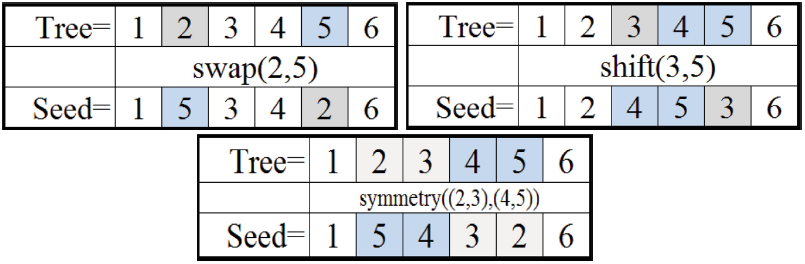
\includegraphics[scale = 0.55]{operations}
    \caption{Examples for the three operations swap, shift, and symmetry. Picture taken from Cinar et al.\cite{cinar20}.}
    \label{fig:operations}
\end{figure}

An example for each operation is given in Figure \ref{fig:operations}.
With \emph{swap} the positions of two given nodes in the path get swapped.
\emph{Shift} is a kind of rotation, where every node in a given interval moves one place to the left except the most left node, which is then set to the right end of the interval.
With \emph{symmetry} the order of nodes in a given interval is reversed to create a mirror image of the interval, effectively changing a subpath from $A-B$ to $B-A$.

The same parameters were used as advised by the paper's authors\cite{cinar20} to make the results comparable.
$max\_fes = 800000$ indicates the number of seeds that are produced overall.
$search\_tendency = 0.5$ indicates the ratio between using the recent tree or the overall best tree for producing the next seed.
$population\_size = number\_of\_cities$ indicates how many seeds are selected for the next iteration.
Details can be found in the original paper by Cinar et al.\cite{cinar20} and pseudocode is provided in the appendix \ref{sec:PseudocodeDTSA}.

\subsection{Implementation of the GA}
For investigating the strengths and weaknesses of the DTSA, a similar genetic algorithm to solve TSPs was implemented and its performance was compared to the DTSA.
At the beginning of the algorithm $number\_of\_cities$ initial solutions are created of which one is created by the nearest neighbor algorithm.
Every solution gets mutated into three new possible solutions by using  swap, shift, and symmetry as described.
Of all solutions the best $number\_of\_cities$ solutions are picked for the next iteration of mutations.
At the end the overall best solution was optimized by the same 2-opt algorithm.

Three different approaches were tested, which differ by the order of the mutation and selection step.
By this it could be investigated if the order of mutation and selection changes the results tremendously.
In GTSPA-SM the solutions are first selected and then mutated. GTSPA-MS has those operations switched, first mutation then selection.
GTSPA-SMS combines these approaches and starts with a selection step, has then a mutation step and finally a selection step.

The proposed evolutionary process is comparable to asexual reproduction because it misses crossover mutations.
These were not implemented, because it is not possible to simply recombine two parts of different \emph{parent trees} to form a new seed, without interfering with the specification of the TSP to visit each city exactly once.

For the number of genes and the maximum function evaluations the same parameters as in the DTSA were used, to ensure a comparability of the algorithms. Pseudocode for the algorithm, which we called GTSPA (short for \emph{Genetic Traveling Salesman Problem Algorithm}), is provided in the appendix \ref{sec:PseudocodeGTSPA}.

\subsection{Experiment setup and statistical evaluation}

The problem instances for the evaluation were taken from tsplib95\cite{tsplib95}.
Six different sets were used ('berlin52', 'st70', 'kroA100', 'eil101', 'ch150' and 'tsp225').
The number at the end of the name gives the number of cities.
Every algorithm was run $n=90$ times for each problem instance.

To compare the different algorithms, different statistical parameters were calculated.
These are the mean $\mu$, standard deviation $\sigma$, and the return error $RE$ which describes the deviation from the optimal solution in percent.
In addition boxplots\cite{Spear52} are used for result visualization for each problem.
The complete formulas of the calculated parameters are given here:

\begin{equation}
	\mu = \frac{1}{n}\sum_{i=1}^{n}x_{i}
\end{equation}

\begin{equation}
	\sigma = \sqrt{\frac{\sum(x_{i}-\mu)^2}{n}}
\end{equation}

\begin{equation}
	RE = \frac{Result - Optimum}{Optimum} \cdot 100
\end{equation}

To calculate the return error, the optimal solutions of the tsplib95 documentation \cite{tsplib95} were used.
The return error was calculated for each sample and then the mean over all samples was calculated.
Also the best and the worst minimum path length over all samples was noted.

%\newpage
\section{Algorithm comparison}
\label{sec:comparison}

To compare the two algorithms, the main focus was the quality of the results.
Because both algorithms are non-deterministic, 90 independent runs were used for evaluation.
The change of the minimum path length was plotted for the different algorithms.
Also the mean and the standard deviation of the minimum path lengths was calculated.
At last the best paths were plotted and compared to the paths of the optimal solutions.
This was done for data sets of different size to see if the performance of the algorithms are dependent on the size of the data set.

\subsection{Change of the path length over iterations}
\label{sec:Change_of_path_length_over_time}

The current minimum path length during the algorithms was plotted over the number of iterations.
It shows the improvement in each iteration, which indicates the convergence rate.
The goal of this investigation was to see which algorithm gets the fastest to a good solution, not to see which one gives the best solution.
For 90 runs of the algorithms the mean of the minimum path length for each iteration was calculated.

\begin{figure}[h]
	\centering
	\begin{subfigure}{.5\textwidth}
		\centering
		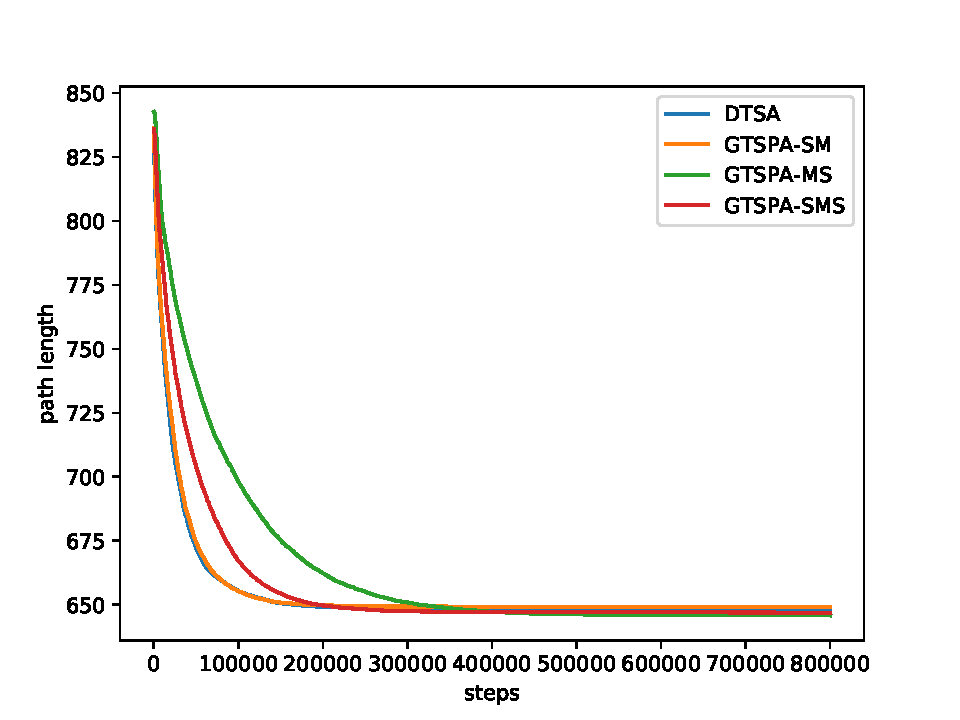
\includegraphics[width=\textwidth]{../../Implementation/gen/mean_convergence_eil101}
		\caption {eil101}
	\end{subfigure}%
	\begin{subfigure}{.5\textwidth}
		\centering
		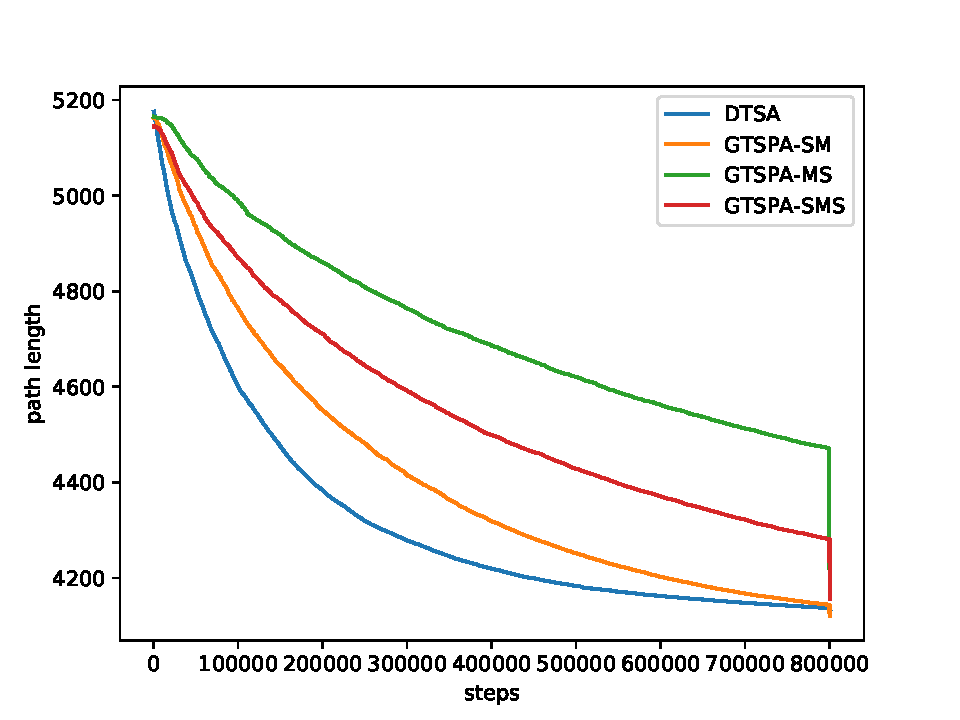
\includegraphics[width=\textwidth]{../../Implementation/gen/mean_convergence_tsp225}
		\caption {tsp225}
	\end{subfigure}
	\caption{Convergence of minimum path length over iterations.}
	\label{fig:mean_convergence_text}
\end{figure}
%\todo[inline]{Student Reviewer 1: (also maybe use different unit to get rid of some zeros)}

Figure \ref{fig:mean_convergence_text} shows, that all algorithms require more iterations with an increasing number of data points.
Individual graphs for four more data sets are provided in the appendix \ref{sec:convergence_of_the_paths}, which underline this observation.
In all analyzed cases, the DTSA is improving the fastest at the beginning, while the GTSPA-MS converges the slowest.
In Figure \ref{fig:mean_convergence_text}(b), which shows the 'tsp225' problem, not all algorithms are fully converged before the stopping criterion is met.
The sharp cut at the end results from the 2-opt algorithm, which decreases the path length rigorously.

\subsection{Final Path Lengths}
\label{sec:final_path_lengths}

The results of the different algorithms for the different problems are analyzed.
Therefore, the mean, standard deviation, and return error (RE) of the final path lengths are calculated.
The results for the six problem instances are shown in Table 1.
Detailed boxplots are are illustrated in appendix \ref{sec:boxplots_for_different_problems}.

\begin{table}[ht]
\begin{center}
\resizebox{\textwidth}{!}{%
\begin{tabular}{|c|c|c|c|c|c|c|}
	\hline
	dataset & algorithm & mean & std. dev. & best & worst & RE(\%)\\
	\hline
	\multirow{4}{*}{berlin52}		& DTSA & 7868.18 & 185.5 & \textbf{7542} & \textbf{8405} & 4.32\\
		& GTSPA-SM & 7867.68 & 193.33 & \textbf{7542} & 8301 & 4.32\\
		& GTSPA-MS & \textbf{7790.32} & 175.78 & \textbf{7542} & 8263 & 3.29\\
		& GTSPA-SMS & 7798.98 & 192.88 & \textbf{7542} & 8281 & 3.41\\
	\hline
	\multirow{4}{*}{st70}		& DTSA & 700.57 & 16.09 & 683 & 738 & 3.79\\
		& GTSPA-SM & 698.26 & 15.3 & \textbf{680} & \textbf{747} & 3.45\\
		& GTSPA-MS & \textbf{695.41} & 13.09 & 682 & 737 & 3.02\\
		& GTSPA-SMS & 695.47 & 12.2 & 682 & 741 & 3.03\\
	\hline
	\multirow{4}{*}{kroA100}		& DTSA & 21831.69 & 382.83 & \textbf{21282} & 23009 & 2.58\\
		& GTSPA-SM & 21754.38 & 355.07 & \textbf{21282}& 23136 & 2.22\\
		& GTSPA-MS & \textbf{21588.57} & 348.82 & \textbf{21282} & 23096 & 1.44\\
		& GTSPA-SMS & 21719.31 & 351.1 & \textbf{21282} & \textbf{23224} & 2.05\\
	\hline
	\multirow{4}{*}{eil101}		& DTSA & 647.76 & 8.45 & \textbf{629} & \textbf{671} & 2.98\\
		& GTSPA-SM & 648.99 & 8.66 & 630 & \textbf{671} & 3.18\\
		& GTSPA-MS & \textbf{645.92} & 7.22 & 631 & 665 & 2.69\\
		& GTSPA-SMS & 646.9 & 8.26 & 630 & 669 & 2.85\\
	\hline
	\multirow{4}{*}{ch150}		& DTSA & 6688.03 & 85.32 & 6549 & \textbf{6922} & 2.45\\
		& GTSPA-SM & 6683.87 & 88.31 & 6549 & 6898 & 2.39\\
		& GTSPA-MS & 6665.89 & 86.8 & 6552 & 6913 & 2.11\\
		& GTSPA-SMS & \textbf{6661.59} & 77.5 & \textbf{6544} & 6839 & 2.05\\
	\hline
	\multirow{4}{*}{tsp225}		& DTSA & 4132.73 & 64.11 & 3995 & \textbf{4365} & 5.45\\
		& GTSPA-SM & \textbf{4121.48} & 57.02 & \textbf{3987} & 4307 & 5.17\\
		& GTSPA-MS & 4188.68 & 55.87 & 4038 & 4350 & 6.88\\
		& GTSPA-SMS & 4156.21 & 54.31 & 4039 & 4330 & 6.05\\
	\hline
\end{tabular}}
\caption{Statistical evaluation of the different algorithms for the six problems. The best results for the columns \textit{mean} and \textit{best} are bold. Also the worst results in the column \textit{worst} are bold.}
\label{table:algo-stats}
\end{center}
\end{table}

The DTSA produces on average the worst results on every problem instance except for 'eil101' and 'tsp225'.
This also applies for the error rate of the DTSA.
The best results of all algorithms are for 'berlin52' and 'kroA100' the optimal solution.
For the other problems the best results are near to each other.
The error rate is the highest for the analyzed problem instance with the largest number of cities.

\subsection{Final Tours}

To evaluate the final solutions in more detail, the best path given by the algorithm was plotted and compared to the optimal path.
The results are included in appendix \ref{sec:final_paths} in Figure \ref{fig:final_paths_berlin52}-\ref{fig:final_paths_tsp225}.
For the 'berlin52' and 'kroA100' problems the results of the four algorithms are identical.
They also correspond to the optimal path as it is shown in Table 1.
For 'st70', 'eil101' and 'ch150' the results of the algorithms have minor differences.
None of the resulting paths matches exactly with the optimal path.

\begin{figure}[ht]
	\begin{subfigure}{.5\textwidth}
		\centering
		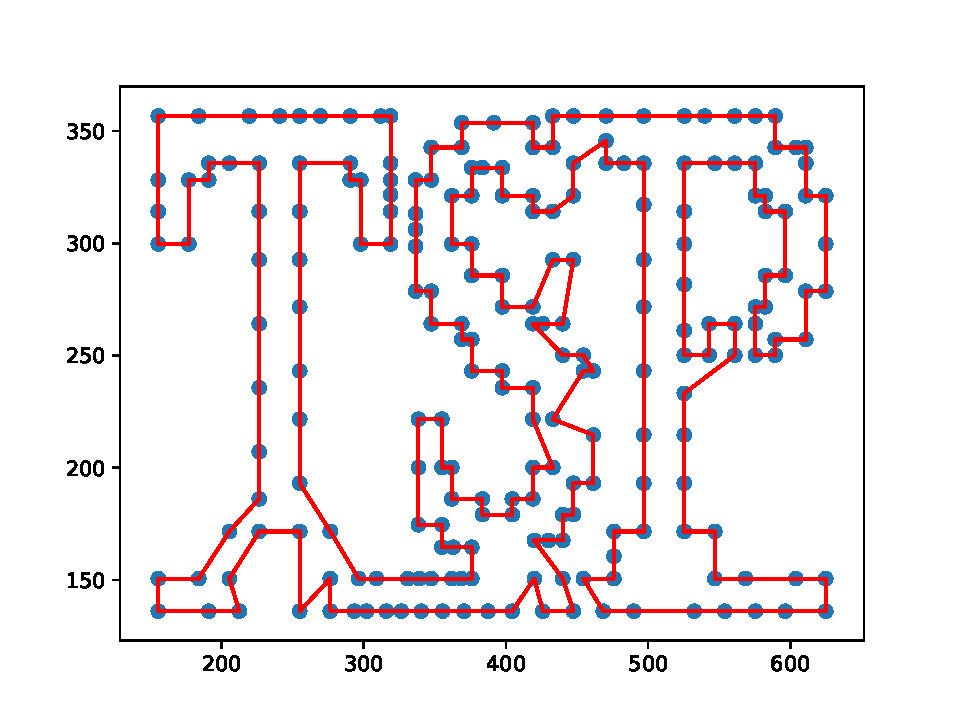
\includegraphics[width=\textwidth]{../../Implementation/gen/best_path_gtspasms_tsp225}
		\caption {GTSPA-SMS}
	\end{subfigure}%
	\begin{subfigure}{.5\textwidth}
		\centering
		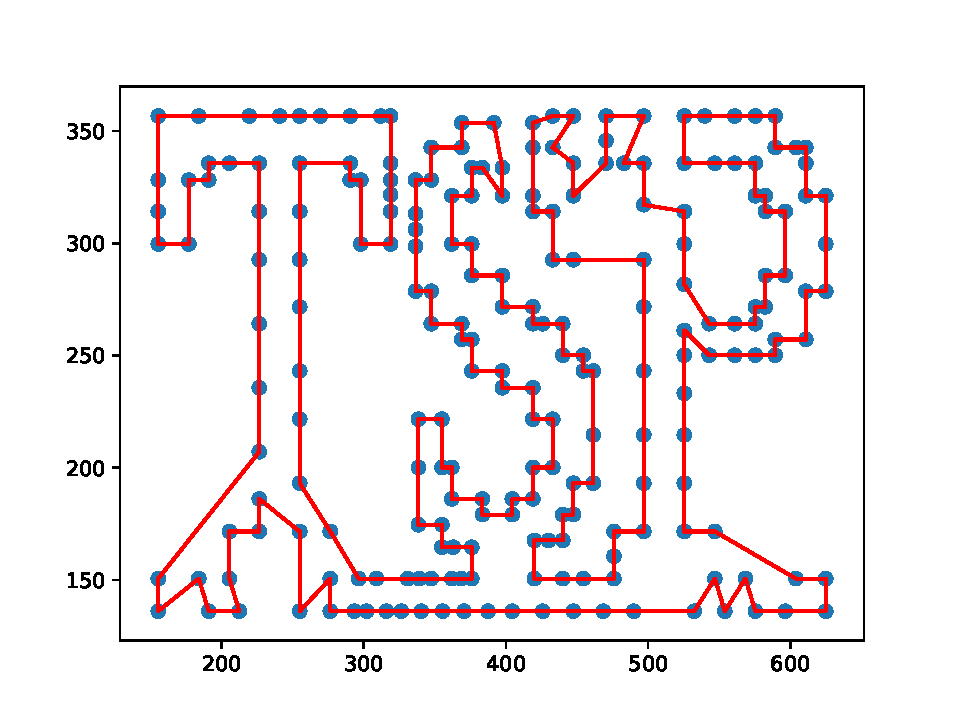
\includegraphics[width=\textwidth]{../../Implementation/gen/best_path_gtspams_tsp225}
		\caption {GTSPA-MS}
	\end{subfigure}
    \caption{Best path for the 'tsp225' problem made with GTSPA-SMS.}
    \label{fig:best_path_tsp225_in_text}
\end{figure}

For the 'tsp225' problem the results are different. The 'T' and the 'P' can be recognized quite good in all figures.
The 'S', which is in the middle of the figures is only noticeable in the GTSPA-SMS and the GTSPA-MS approach (Figure \ref{fig:best_path_tsp225_in_text}).
Interestingly, although for the human mind the best results of these two algorithms look quite similar to the optimal solution, they produced the longer best paths (GTSPA-SMS = 4039, GTSPA-MS = 4038) in comparison to the other two algorithms (DTSA = 3995, GTSPA-SM = 3987) as it can be noticed in Table \ref{table:algo-stats}.

%\newpage
\section{Discussion}
\label{sec:discussion}

As it was described in Section \ref{sec:Change_of_path_length_over_time}, the DTSA converges to local minima faster compared to the other algorithms.
But this usually only has an impact on the run time and not on the result, because of the 2-opt algorithm, which is executed at the end.
This can be seen in Figure \ref{fig:mean_convergence_text} in the 'tsp225' plot.
Though the DTSA being faster, it gives a little bit worse final solutions on average.
It has the highest mean for all analyzed problems except for 'eil101' where it is third best and 'tsp225' where it has the second best mean.
On considerably smaller problems, all algorithms give the same best solution as it was the case for 'berlin52' and 'kroA100'.

The results of the algorithms only differ slightly from each other.
Therefore, similarities and differences of the algorithms were also examined to analyze the relationship of the DTSA to a genetic algorithm.
In the implementation all algorithms use the same operations (swap, shift and symmetry).
Also the concept of selection is evident in the DTSA.
This could be the reason for the similar results, that the algorithms have these structural similarities.
The only difference is that the DTSA is missing is a crossover operation.
However, the usage of $best$ and $random$ instead of only the $current$ tree to generate new seeds, could be considered as a kind of crossover.
It does not mix parts of each solutions to make a new one, but replace one completely by the other, like a crossover which starts at the first base of a chromosome.

Three different variants of the GTSPA were tested, which only differ by the order of the mutation and selection step.
This was done to test if the different approaches would differ from each other significantly.
It can be seen in Figure \ref{fig:mean_convergence_text} that the GTSPA-SM is most of the time the fastest, while the GTSPA-MS approach takes the most steps to reach the final best path.
If given enough time, the GTSPA-MS returns the best average result.
A reason for this could be the fact that the different order of the mutation and selection approach only result in different population sizes and therefore lead to different exploration spaces.
This leads to the GTSPA-SM having the smallest population during the process of mutation while GTSPA-MS has the largest.
The same variants of the algorithms could be achieved by changing only the starting population sizes.
A greater population size means a more explored solution space (better results) but also less iterations overall (slower convergence, more time needed).

The implemented algorithms returned overall quite good results, but they also have some limitations.
In this case only six rather small problem instances were used.
As described in Section \ref{sec:final_path_lengths} the algorithms perform better on smaller instances.
Real world applications include often more than 225 cities, which would lead to worse results.
Also in the real world asymmetric TSPs are more common.
A possible way to solve asymmetric TSPs could be to transform them into symmetric TSPs.
Jonker and Volgenant (1983) presented a way to perform this transformation\cite{ATSP1}.
Their idea was to create a $2n \times 2n$ distance matrix, with so called ghost nodes.
These ghost nodes need to be included in the optimal solution.
With this approach both distances between two cities can be denoted.
A $3 \times 3$ example of this approach is given in Figure \ref{fig:ATSP_example}.

\begin{figure}[ht]
    \centering
    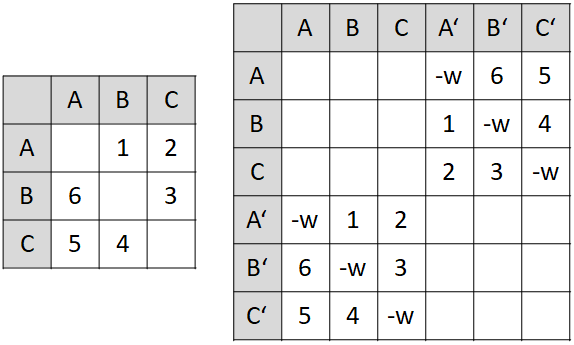
\includegraphics[scale = 0.4]{ATSP}
    \caption{Example of the approach to convert an ATSP into a TSP.}
    \label{fig:ATSP_example}
\end{figure}

A possible solution would be $A \rightarrow A' \rightarrow C \rightarrow C' \rightarrow B \rightarrow B' \rightarrow A$.
As it can be seen the path goes first to the corresponding ghost node before it continues to the next city.
This is a necessity to be able to derive a path from the solution.
With this approach the implemented DTSA and GAs can be used to calculate asymmetric TSPs, but it needs more time.
A problem might be, that the ghost nodes need to be connected to their respective real node.
This can not be ensured with the mutation operations and the 2-opt algorithm.
A lot of testing with the weight between the nodes and their ghost nodes would be required.
Other special issues of this approach are discussed in the corresponding paper\cite{ATSP2}.

Although theoretically the implemented algorithms could be used to solve asymmetric TSPs as well, they only perform well on symmetric ones.
Both algorithms rely on small changes of the best trees, performed by the operations swap, shift and symmetry.
While these operations (especially symmetry) can already have a major impact on the solutions, most of the time only small changes are made between the iterations.
In an asymmetric TSP already a small operation like swap can change the solution a lot, for better or for worse.
This problem might lead to not applying said changes for the next generation, although it could bring even better results in later generations.

%\newpage

\section{Conclusion}
\label{sec:conclusion}

We have implemented the DTSA and a similar GA that uses the same mutation operations to solve TSPs.
Both algorithms were tested with different problem sizes.
We have shown that on average our GTSPA got better results in form of slightly shorter paths.
However the DTSA converged faster to a solution, therefore it is useful if the task is more time-sensitive.
Overall it is recommended to run all algorithms several times and pick the best solution of all runs.
This is a better approach than running the algorithms for more iterations.
At some point the path does not get any shorter although it is not the optimal path, as it can be seen for the smaller problems.
This could be because it is stuck in a local minimum.

The GTSPA was tested with three different orders of selection and mutation to test its influence on the algorithms performance.
This lead to different population sizes during the mutation step and the same variants of the algorithm could be achieved by only using different starting population size.
We found that the GTSPA-SM converges faster on all problems while the GTSPA-MS needs more time, but also leads to better results on average when enough time is provided.

The DTSA is a genetic algorithm in disguise, because it follows a similar approach and uses the same operations.
On average it can provide solutions in fewer generations than the GTSPA, but provides worse solutions that result in longer paths.

The algorithms could be applied to solve real world problems, but will probably face some limitations.
A problem with 225 cities could be solved, but with more cites the run time increases exponentially.
Also asymmetric TSPs are more often seen in real world application.
A solution to solve these was presented, but will again increase the computational costs and running time.

\newpage
\bibliography{bib}
\bibliographystyle{unsrt}

\newpage

\section{Appendix}

\subsection{Pseudocode DTSA}
\label{sec:PseudocodeDTSA}

The following lines describe the discrete tree-seed algorithm.

\begin{algorithm}[H]
	\DontPrintSemicolon
	\SetAlgoLined
	\KwData {$maxfes$, $numcities$, $numtrees$, $searchtendency$, }
	\KwResult {Hamiltonian circle}
	\Begin{
		Set first tree as nearest neighbor tour\;
		Create $numtrees-1$ trees as random permutation between 1 and $numcities$\;
		Set $fes$ to $numtrees$\;
		Set $best$ to tree with shortest tour\;
		\While{$fes$ $<$ $maxfes$}{
			\For{$current$ in all trees}{
				Get $random$ tree (except $current$)\;
				Set $rand$ to random number between 0 and 1\;
				\eIf{$rand$ $<$ $searchtendency$} {
					Create seed with \FuncSty{swap($best$)}\;
					Create seed with \FuncSty{shift($best$)}\;
					Create seed with \FuncSty{symmetry($best$)}\;
					} {
					Create seed with \FuncSty{swap($current$)}\;
					Create seed with \FuncSty{shift($current$)}\;
					Create seed with \FuncSty{symmetry($current$)}\;
				}
				Create seed with \FuncSty{swap($random$)}\;
				Create seed with \FuncSty{shift($random$)}\;
				Create seed with \FuncSty{symmetry($random$)}\;
				$fes$ $+=$ $6$\;
				Set $bestseed$ to seed with shortest tour\;
				\If{$bestseed$ $<$ $current$} {
					Set $current$ to $bestseed$\;
				}
			Set $best$ to tree with shortest tour\;
			}
		}
		Set $best$ to \FuncSty{2-opt($best$)}\;
		\KwRet{$best$}\;
	}
	\caption{Discrete tree-seed algorithm}
\end{algorithm}

\newpage

\subsection{Pseudocode GTPSA}
\label{sec:PseudocodeGTSPA}

The following lines describe the genetic algorithm.

\begin{algorithm}[H]
	\DontPrintSemicolon
	\SetAlgoLined
	\KwData {$maxfes$, $numcities$, $numtrees$, $preselection$, }
	\KwResult {Hamiltonian circle}
	\Begin{
		Set $k$ to $numtrees \cdot preselection$\;
		Set first tree as nearest neighbor tour\;
		Create $numtrees-1$ trees as random permutation between 1 and $numcities$\;
		Set $fes$ to $numtrees$\;
		Set $best$ to tree with shortest tour\;
		\While{$fes$ $<$ $maxfes$}{
			Get best $k$ trees with shortest tour\;
			Initialize next generation of trees as an empty list $possiblenext$\;
			\For{$current$ in $k$ best trees}{
				Create seed with \FuncSty{swap($current$)}\;
				Create seed with \FuncSty{shift($current$)}\;
				Create seed with \FuncSty{symmetry($current$)}\;
				$fes$ $+=$ $3$\;				
			Get best $numtrees$ trees of $possiblenext$ with shortest tour\;
			}
		Set $best$ to tree with shortest tour\;
		}
	Set $best$ to \FuncSty{2-opt($best$)}\;
	\KwRet{$best$}\;
	}
	\caption{genetic algorithm}
\end{algorithm}

\newpage

\subsection{Convergence of the paths}
\label{sec:convergence_of_the_paths}

Convergence of the algorithms for different data sets by increasing size.

\begin{figure}[h]
	\centering
	\begin{subfigure}{.5\textwidth}
		\centering
		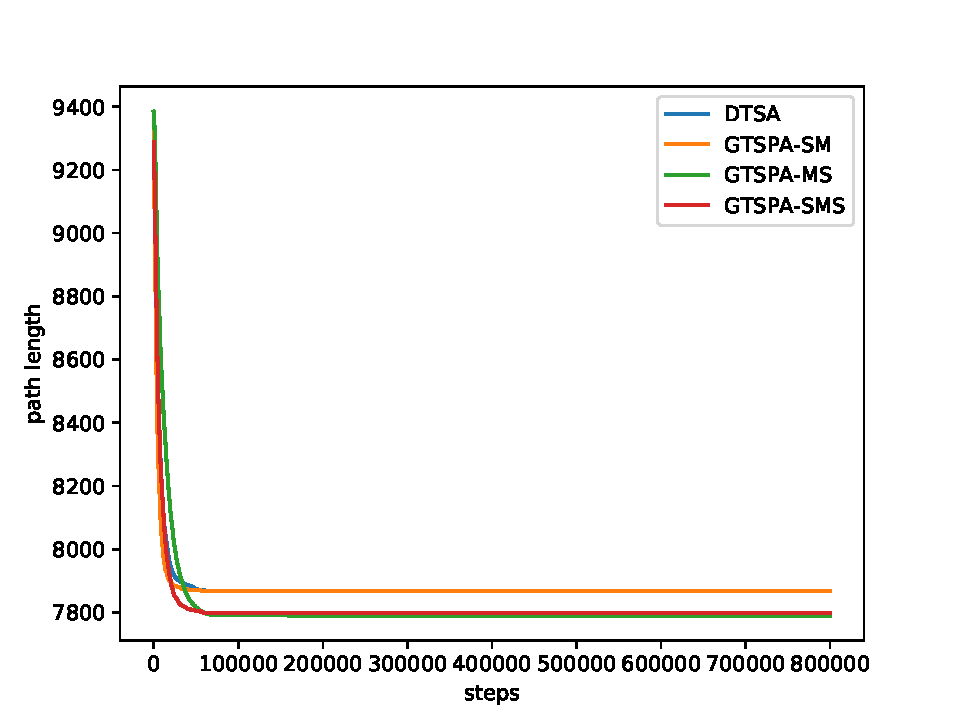
\includegraphics[width=\textwidth]{../../Implementation/gen/mean_convergence_berlin52}
		\caption{berlin52}
	\end{subfigure}%
	\begin{subfigure}{.5\textwidth}
		\centering
		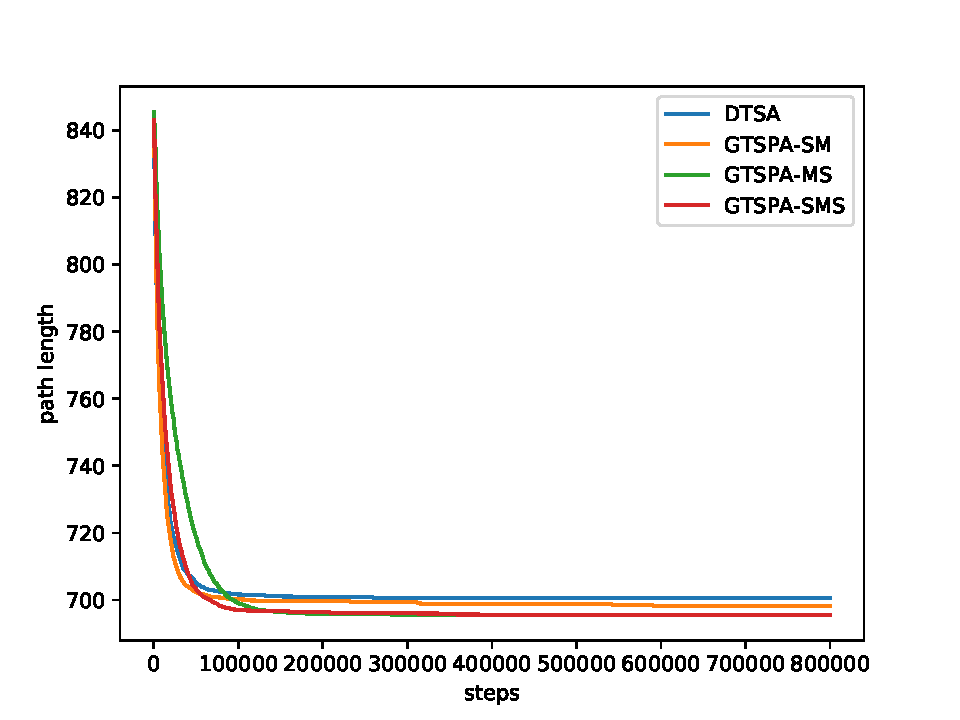
\includegraphics[width=\textwidth]{../../Implementation/gen/mean_convergence_st70}
		\caption{st70}
	\end{subfigure}
	\begin{subfigure}{.5\textwidth}
		\centering
		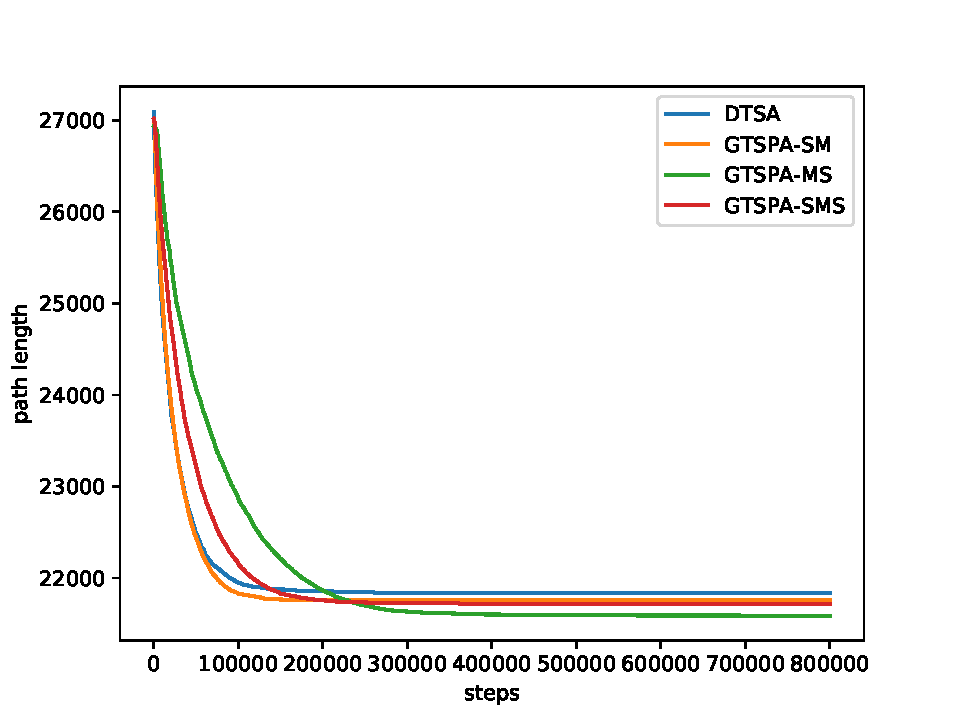
\includegraphics[width=\textwidth]{../../Implementation/gen/mean_convergence_kroA100}
		\caption{kroA100}
	\end{subfigure}%
	\begin{subfigure}{.5\textwidth}
		\centering
		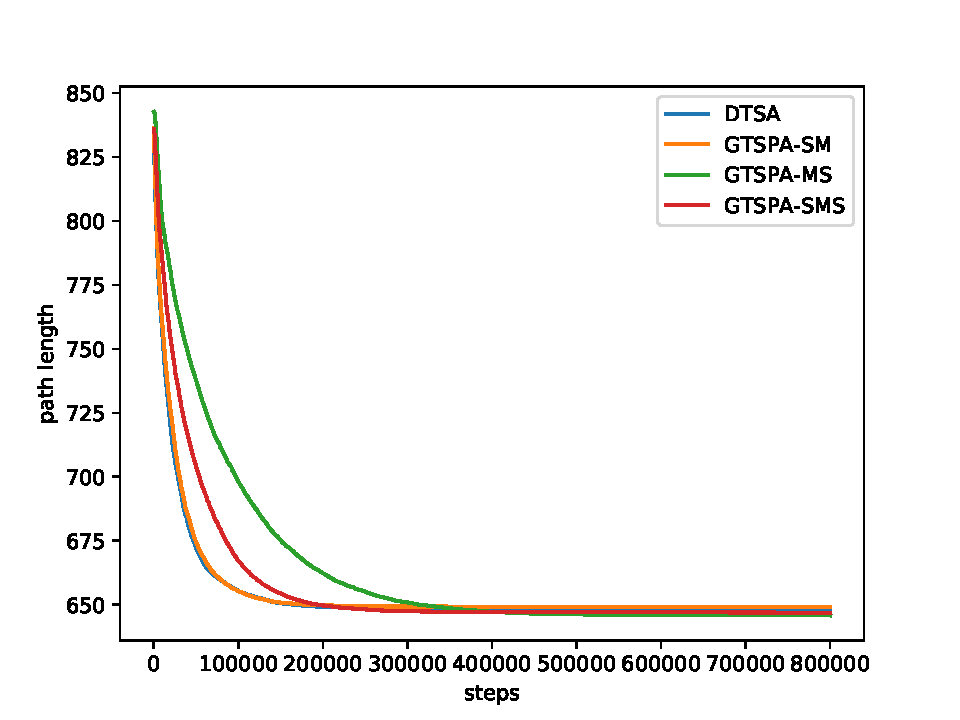
\includegraphics[width=\textwidth]{../../Implementation/gen/mean_convergence_eil101}
		\caption{eil101}
	\end{subfigure}
	\begin{subfigure}{.5\textwidth}
		\centering
		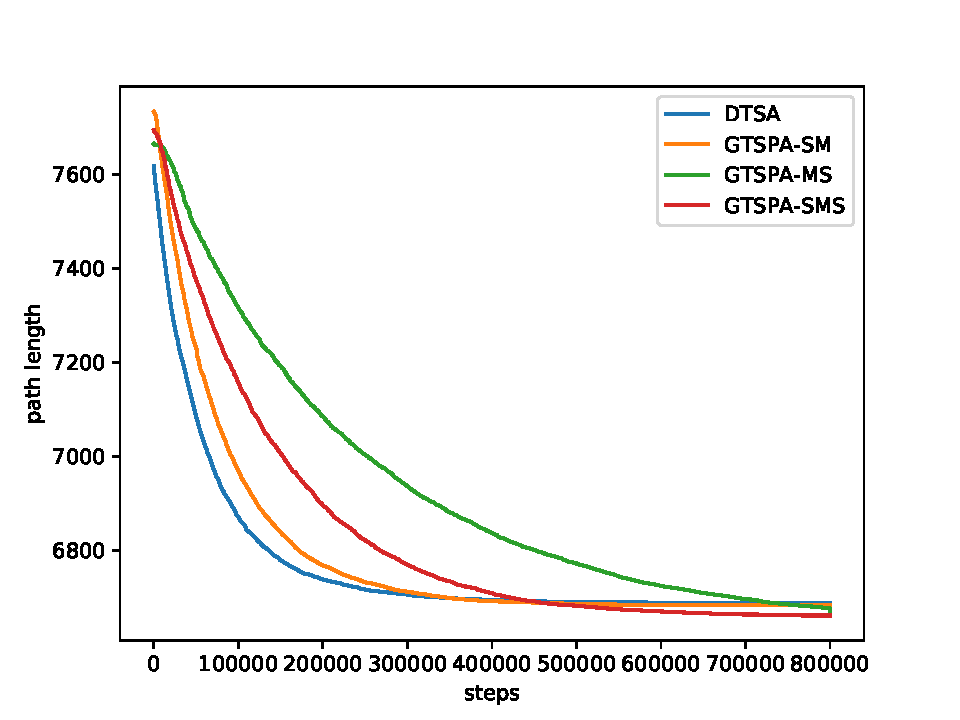
\includegraphics[width=\textwidth]{../../Implementation/gen/mean_convergence_ch150}
		\caption{ch150}
	\end{subfigure}%
	\begin{subfigure}{.5\textwidth}
		\centering
		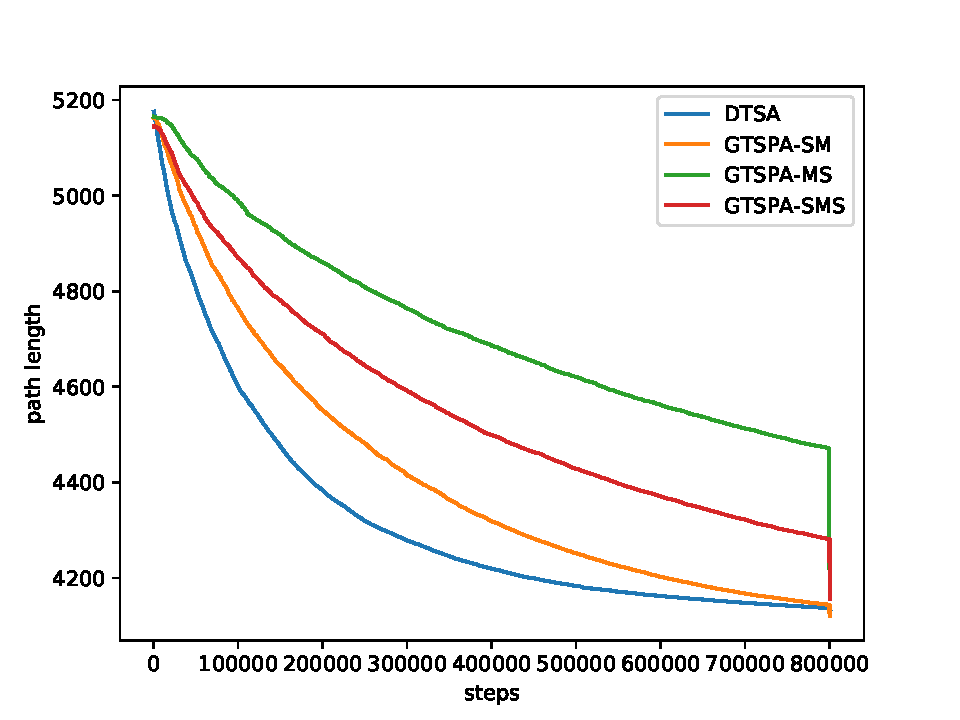
\includegraphics[width=\textwidth]{../../Implementation/gen/mean_convergence_tsp225}
		\caption{tsp225}
	\end{subfigure}
	\caption{Convergence of minimum path length over time.}
	\label{fig:mean_convergence}
\end{figure}

\newpage

\subsection{Boxplots for different problems}
\label{sec:boxplots_for_different_problems}

Boxplots different problem instances by increasing size.

\begin{figure}[h]
	\centering
	\begin{subfigure}{.5\textwidth}
		\centering
		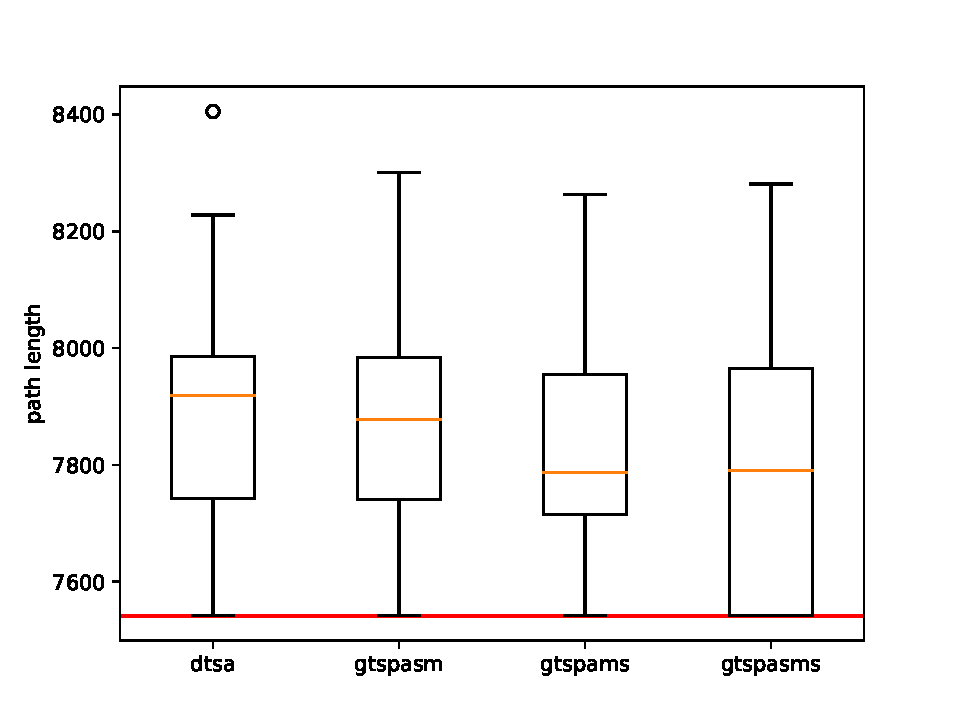
\includegraphics[width=\textwidth]{../../Implementation/gen/boxplot_berlin52}
		\caption{berlin52}
	\end{subfigure}%
	\begin{subfigure}{.5\textwidth}
		\centering
		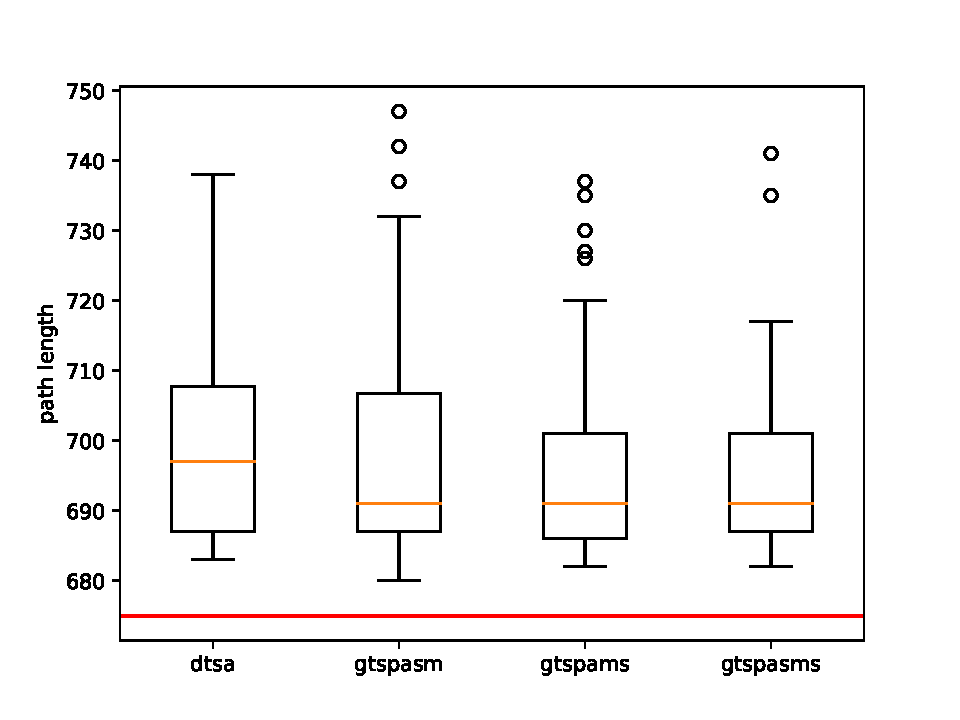
\includegraphics[width=\textwidth]{../../Implementation/gen/boxplot_st70}
		\caption{st70}
	\end{subfigure}
	\begin{subfigure}{.5\textwidth}
		\centering
		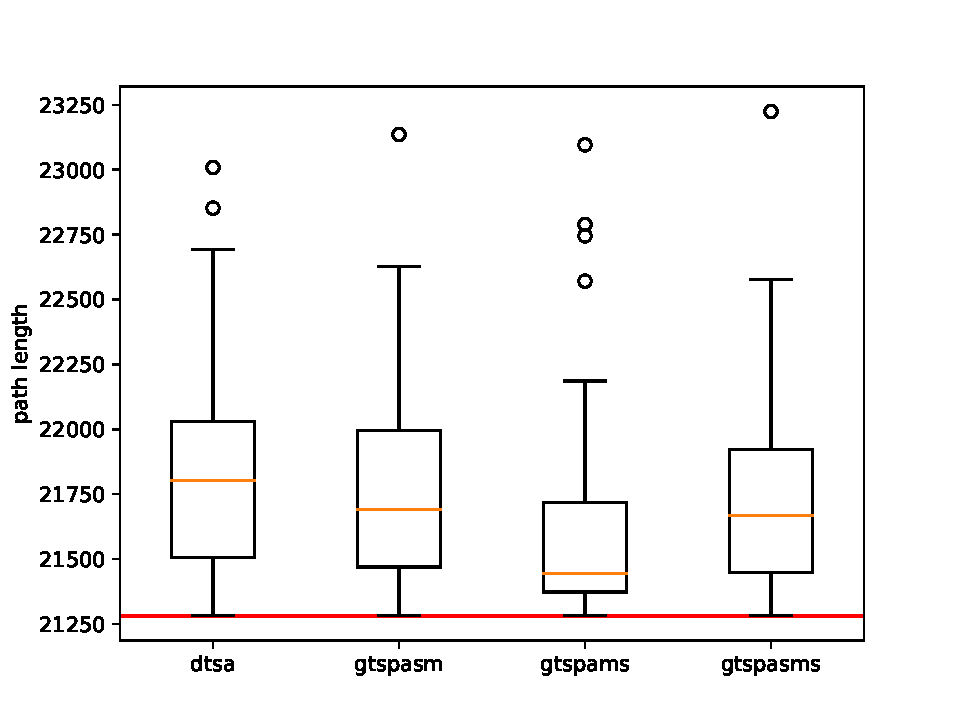
\includegraphics[width=\textwidth]{../../Implementation/gen/boxplot_kroA100}
		\caption{kroA100}
	\end{subfigure}%
	\begin{subfigure}{.5\textwidth}
		\centering
		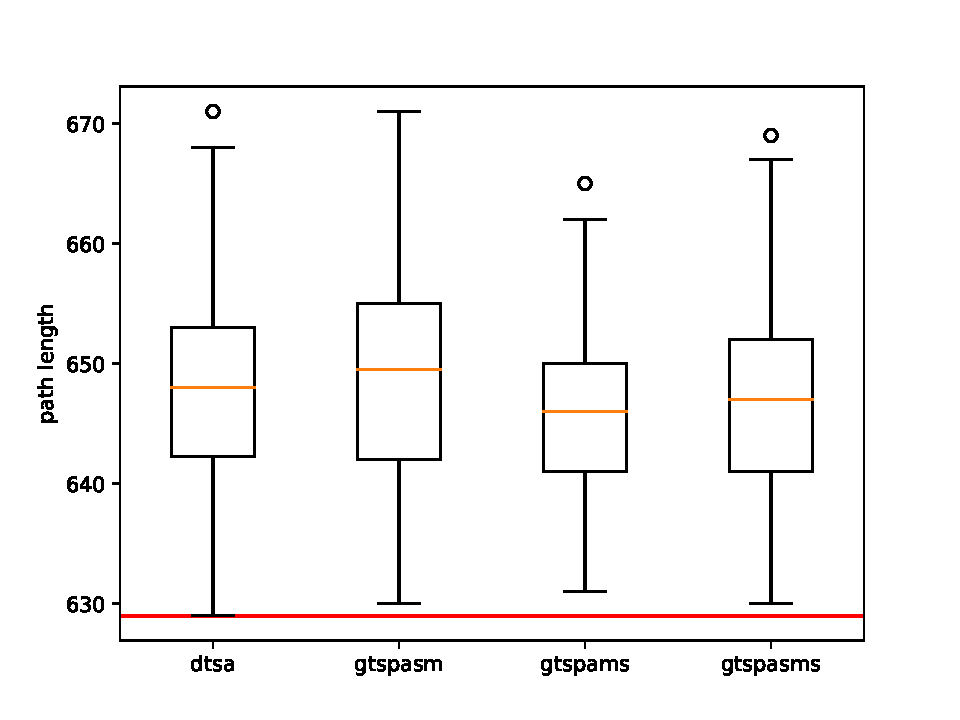
\includegraphics[width=\textwidth]{../../Implementation/gen/boxplot_eil101}
		\caption{eil101}
	\end{subfigure}
	\begin{subfigure}{.5\textwidth}
		\centering
		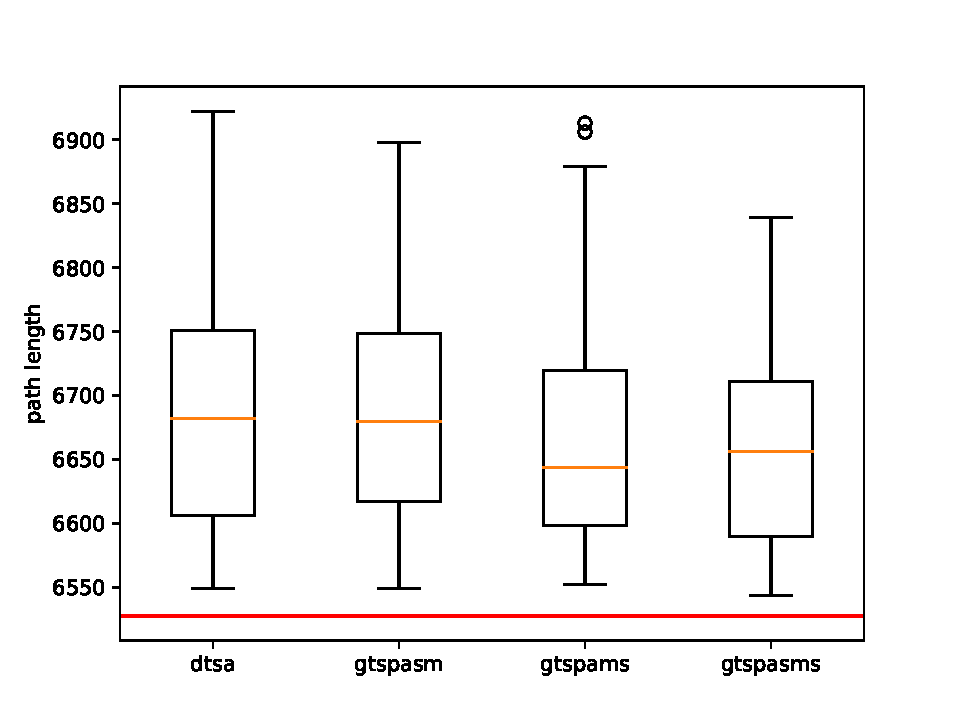
\includegraphics[width=\textwidth]{../../Implementation/gen/boxplot_ch150}
		\caption{ch150}
	\end{subfigure}%
	\begin{subfigure}{.5\textwidth}
		\centering
		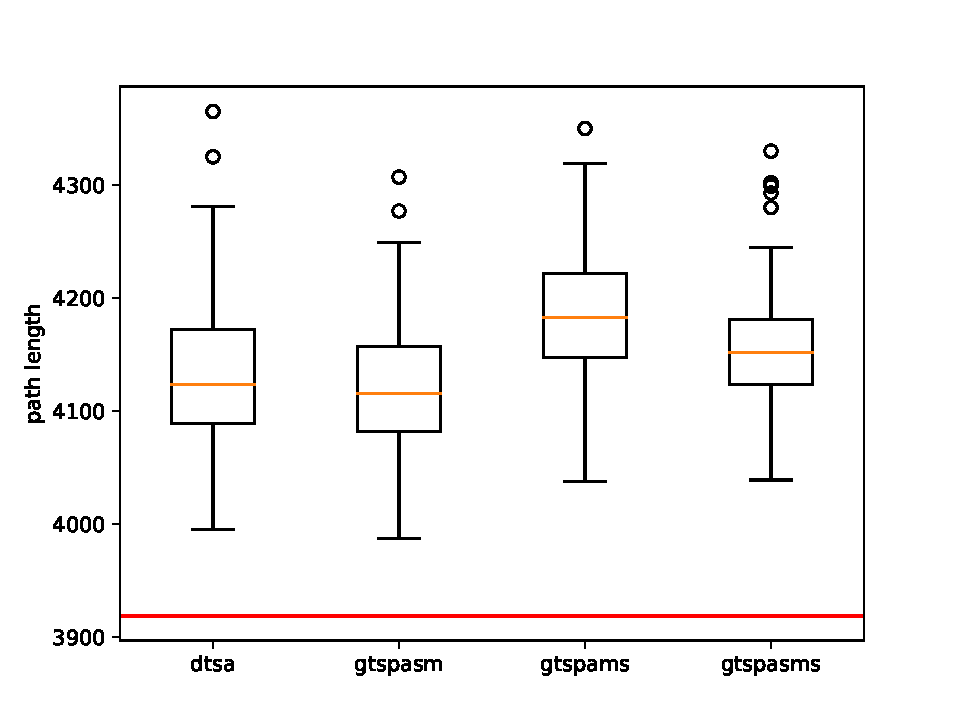
\includegraphics[width=\textwidth]{../../Implementation/gen/boxplot_tsp225}
		\caption{tsp225}
	\end{subfigure}
	\caption{Boxplots with four different algorithms for each problem instance.}
	\label{fig:boxplots}
\end{figure}

\subsection{Final paths}
\label{sec:final_paths}

The final paths for all problems and algorithms are given.

\begin{figure}[ht]
	\centering
	\begin{subfigure}{.5\textwidth}
		\centering
		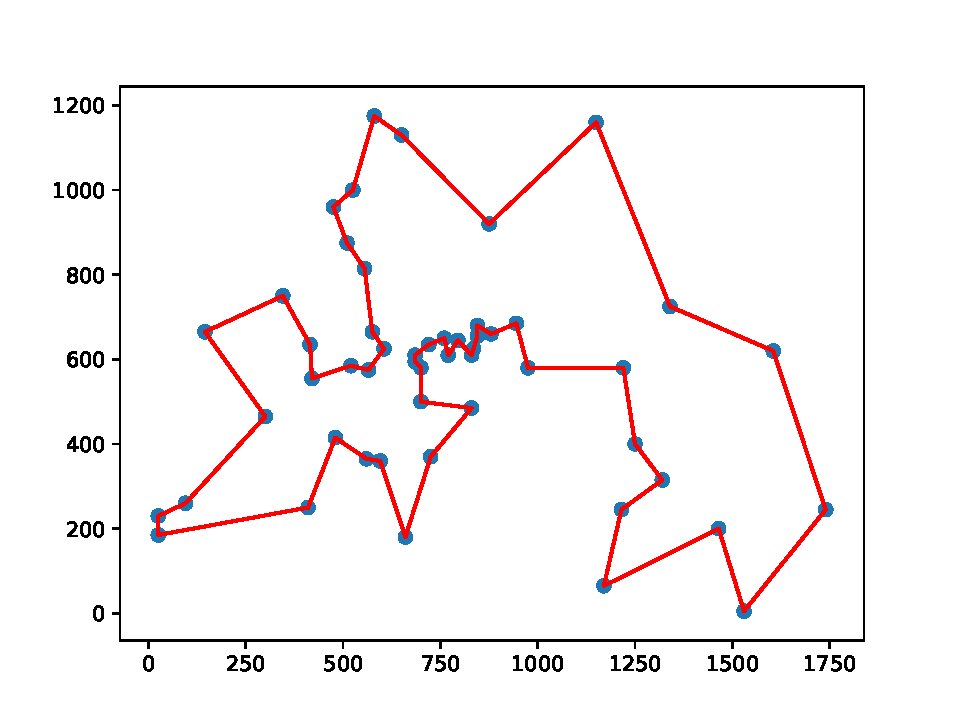
\includegraphics[scale = 0.44]{../../Implementation/gen/best_path_dtsa_berlin52}
		\label{fig:best_path_dtsa_berlin52}
		\caption{DTSA}
	\end{subfigure}%
	\begin{subfigure}{.5\textwidth}
		\centering
		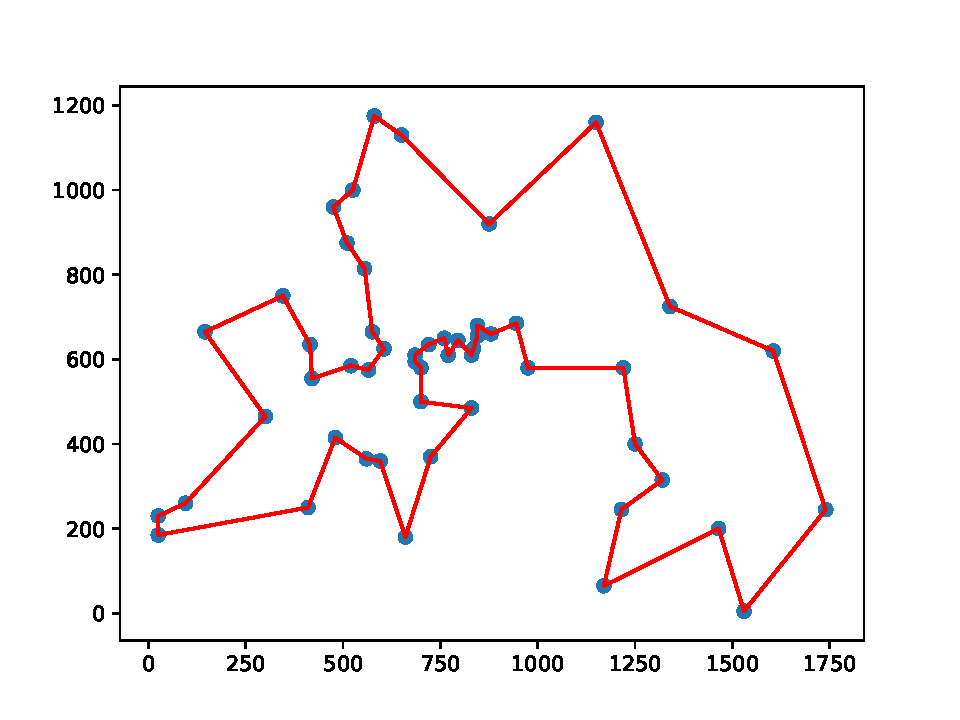
\includegraphics[scale = 0.44]{../../Implementation/gen/best_path_gtspams_berlin52}
		\label{fig:best_path_gtspams_berlin52}
		\caption{GTSPA-MS}
	\end{subfigure}
	\begin{subfigure}{.5\textwidth}
		\centering
		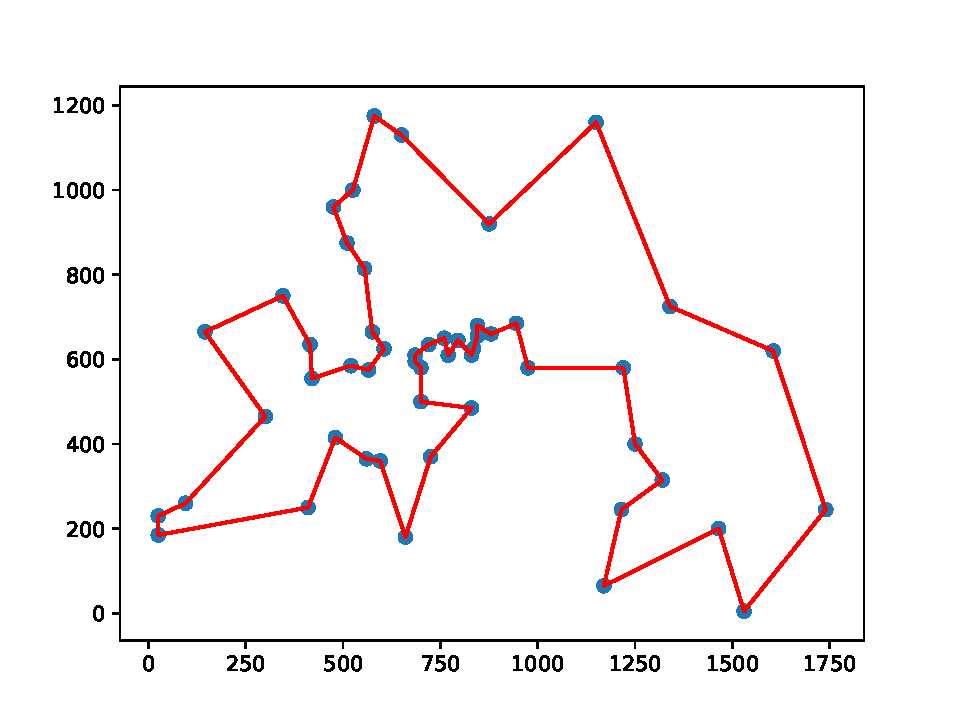
\includegraphics[scale = 0.44]{../../Implementation/gen/best_path_gtspasm_berlin52}
		\label{fig:best_path_gtspasm_berlin52}
		\caption{GTSPA-SM}
	\end{subfigure}%
	\begin{subfigure}{.5\textwidth}
		\centering
		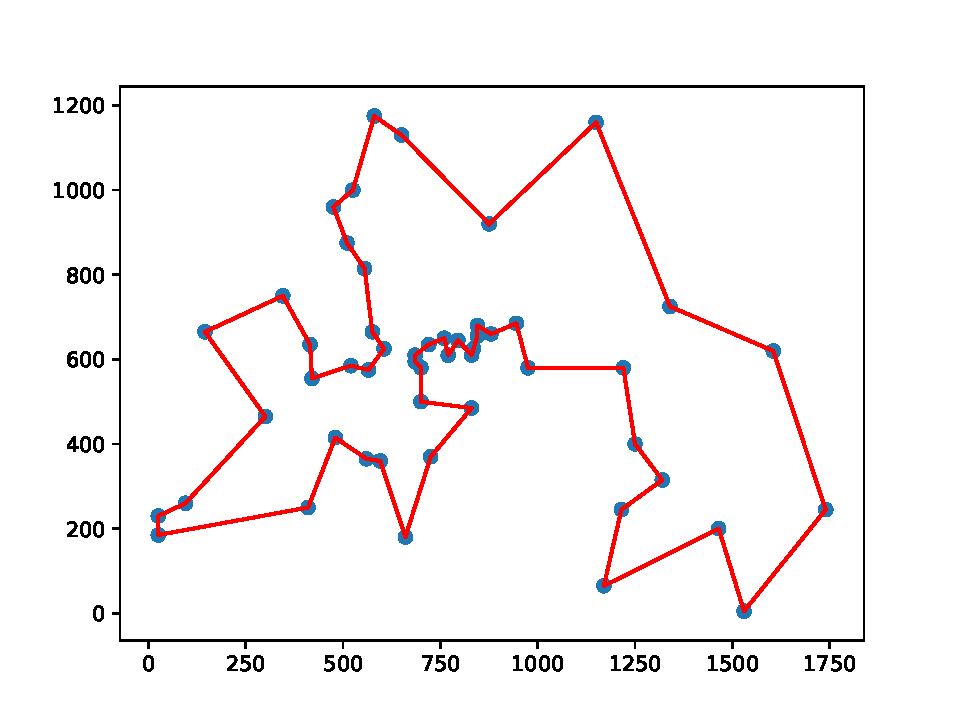
\includegraphics[scale = 0.44]{../../Implementation/gen/best_path_gtspasms_berlin52}
		\label{fig:best_path_gtspasms_berlin52}
		\caption{GTSPA-SMS}
	\end{subfigure}
	\begin{subfigure}{.5\textwidth}
		\centering
		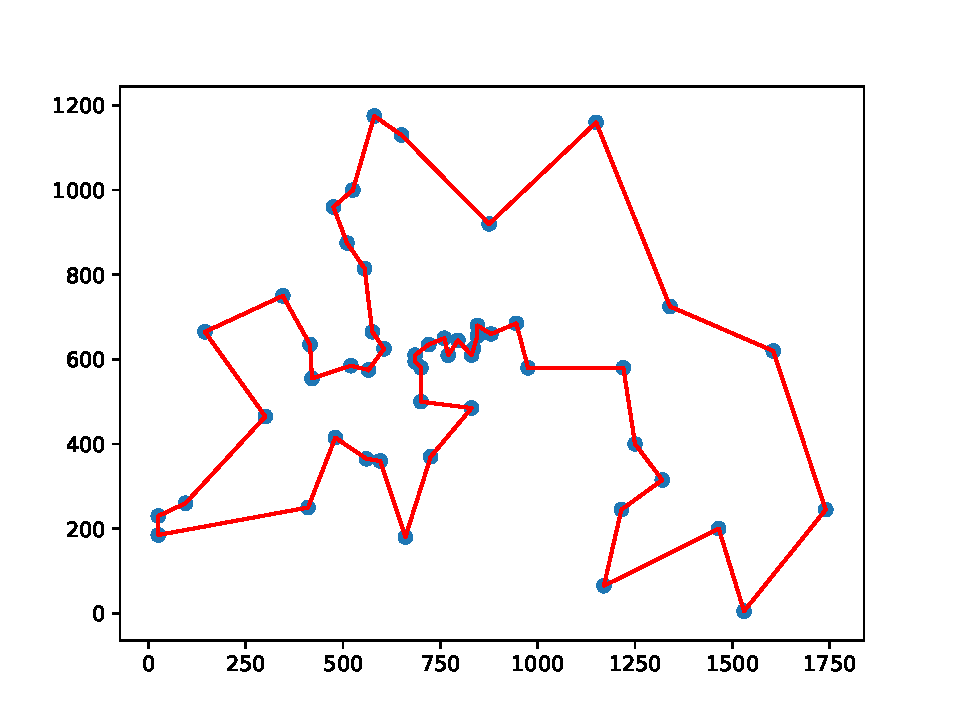
\includegraphics[scale = 0.44]{../../Implementation/gen/optimal_path_berlin52}
		\label{fig:optimal_path_berlin52}
		\caption{optimal path}
	\end{subfigure}
	\caption{Final best paths for the different algorithms and optimal path for 'berlin52' problem.}
	\label{fig:final_paths_berlin52}
\end{figure}
\newpage
\begin{figure}[ht]
	\centering
	\begin{subfigure}{.5\textwidth}
		\centering
		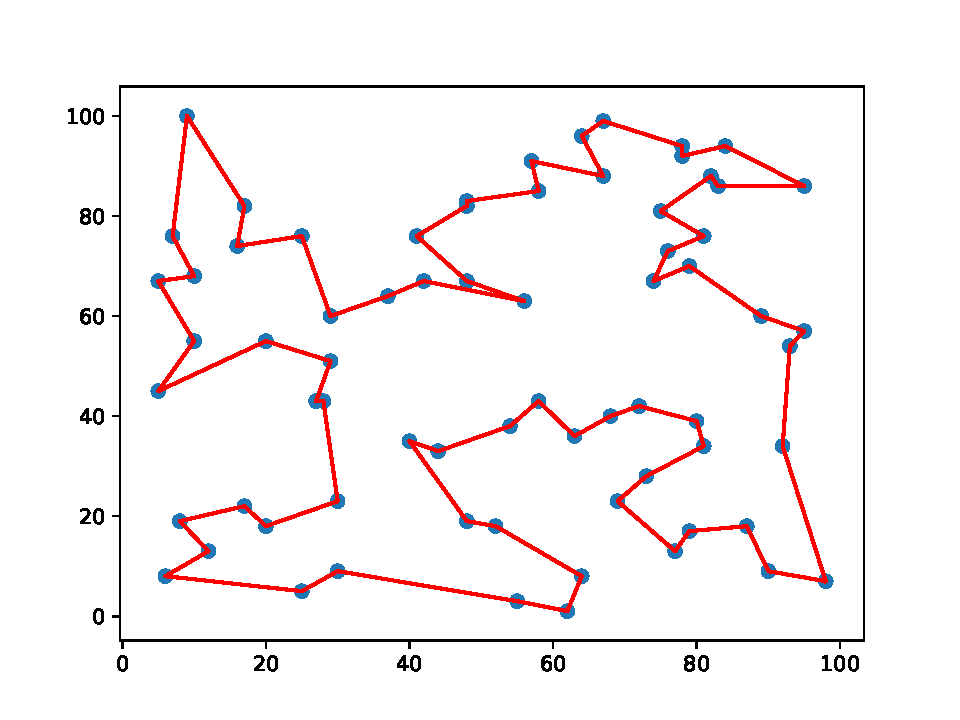
\includegraphics[scale = 0.44]{../../Implementation/gen/best_path_dtsa_st70}
		\label{fig:best_path_dtsa_st70}
		\caption{DTSA}
	\end{subfigure}%
	\begin{subfigure}{.5\textwidth}
		\centering
		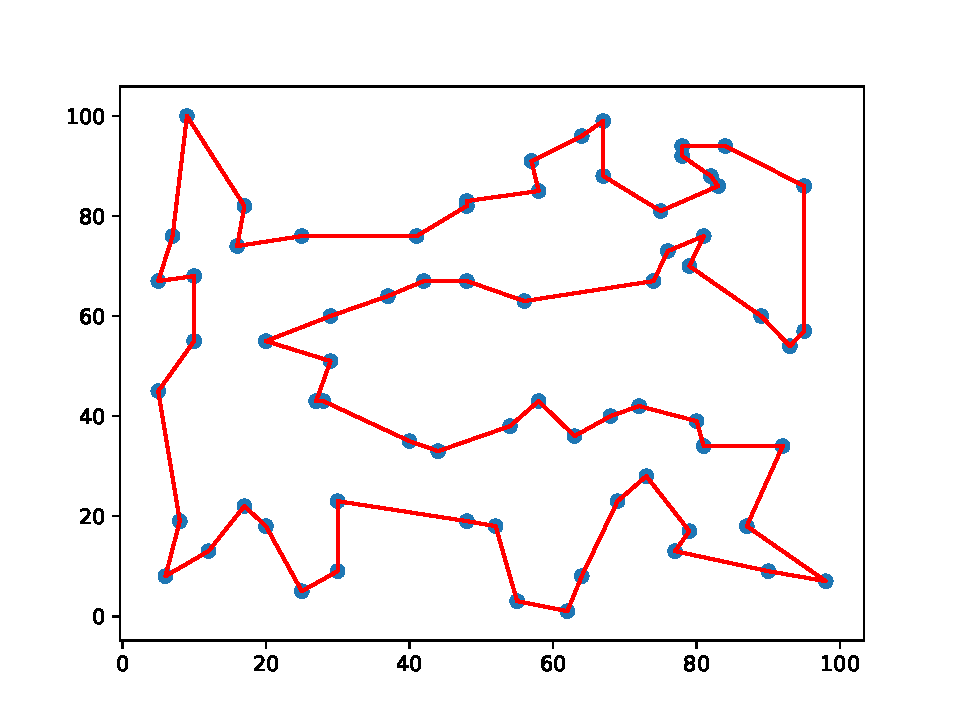
\includegraphics[scale = 0.44]{../../Implementation/gen/best_path_gtspams_st70}
		\label{fig:best_path_gtspams_st70}
		\caption{GTSPA-MS}
	\end{subfigure}
	\begin{subfigure}{.5\textwidth}
		\centering
		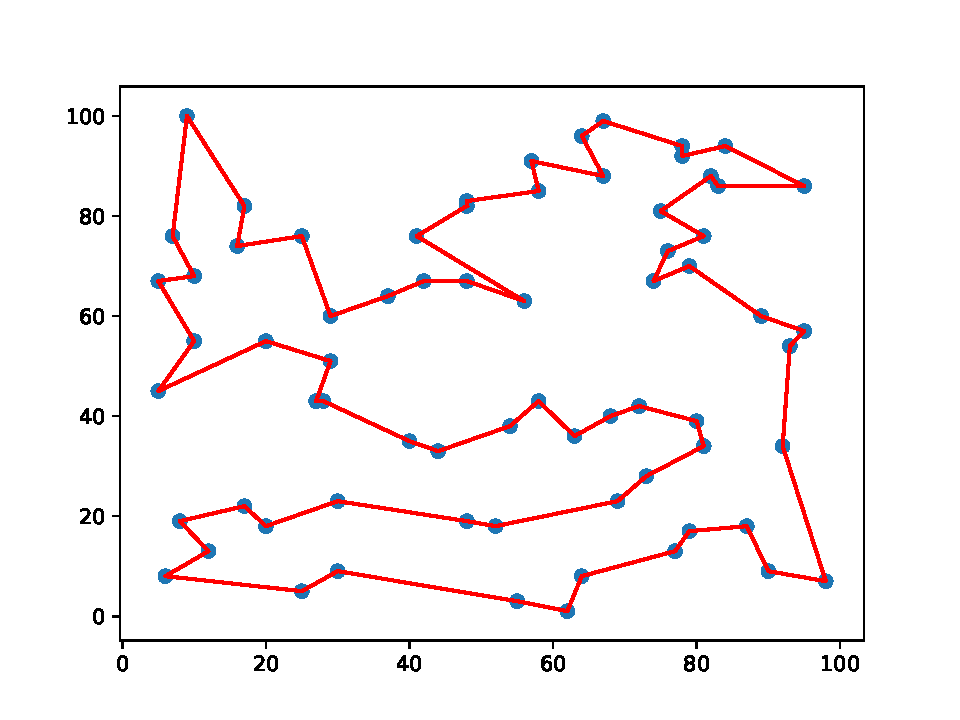
\includegraphics[scale = 0.44]{../../Implementation/gen/best_path_gtspasm_st70}
		\label{fig:best_path_gtspasm_st70}
		\caption{GTSPA-SM}
	\end{subfigure}%
	\begin{subfigure}{.5\textwidth}
		\centering
		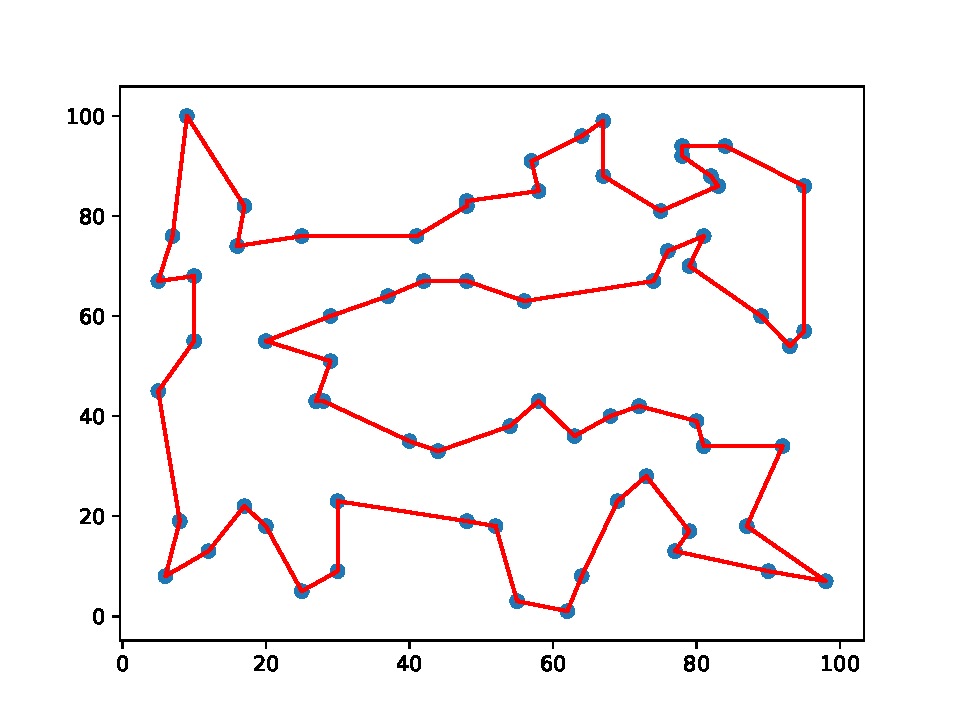
\includegraphics[scale = 0.44]{../../Implementation/gen/best_path_gtspasms_st70}
		\label{fig:best_path_gtspasms_st70}
		\caption{GTSPA-SMS}
	\end{subfigure}
	\begin{subfigure}{.5\textwidth}
		\centering
		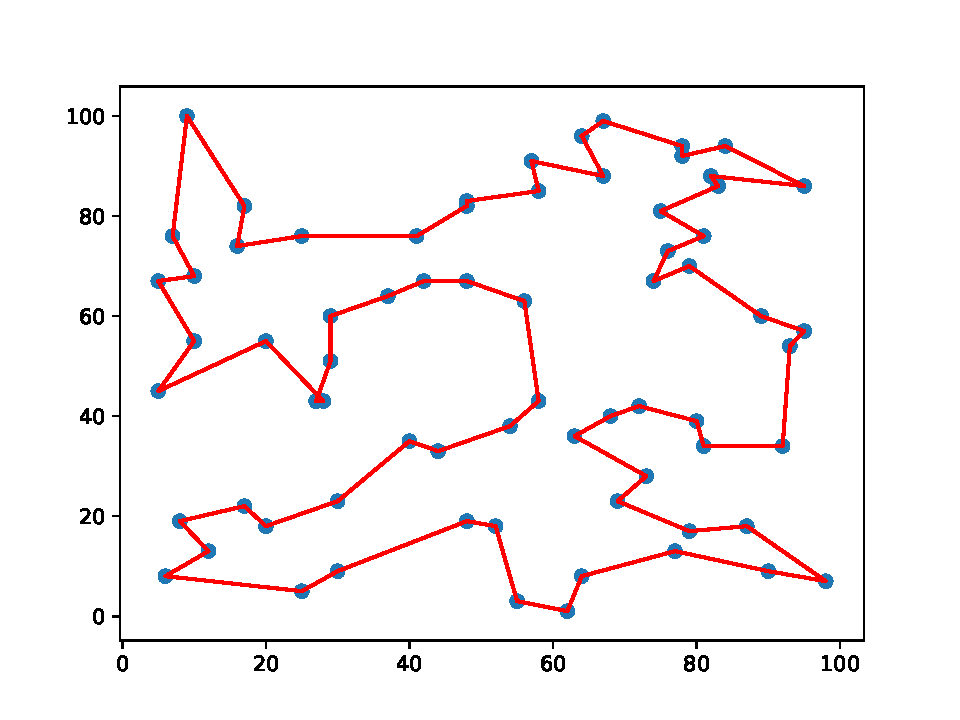
\includegraphics[scale = 0.44]{../../Implementation/gen/optimal_path_st70}
		\label{fig:optimal_path_st70}
		\caption{optimal path}
	\end{subfigure}
	\caption{Final best paths for the different algorithms and optimal path for 'st70' problem.}
	\label{fig:final_paths_st70}
\end{figure}
\newpage
\begin{figure}[ht]
	\centering
	\begin{subfigure}{.5\textwidth}
		\centering
		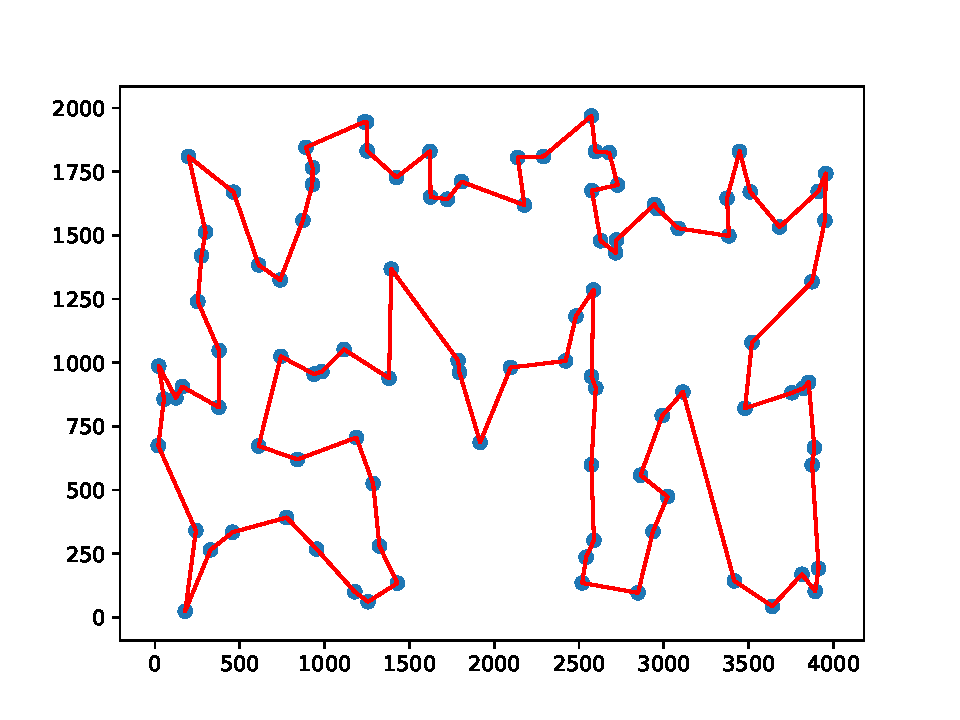
\includegraphics[scale = 0.44]{../../Implementation/gen/best_path_dtsa_kroA100}
		\label{fig:best_path_dtsa_kroA100}
		\caption{DTSA}
	\end{subfigure}%
	\begin{subfigure}{.5\textwidth}
		\centering
		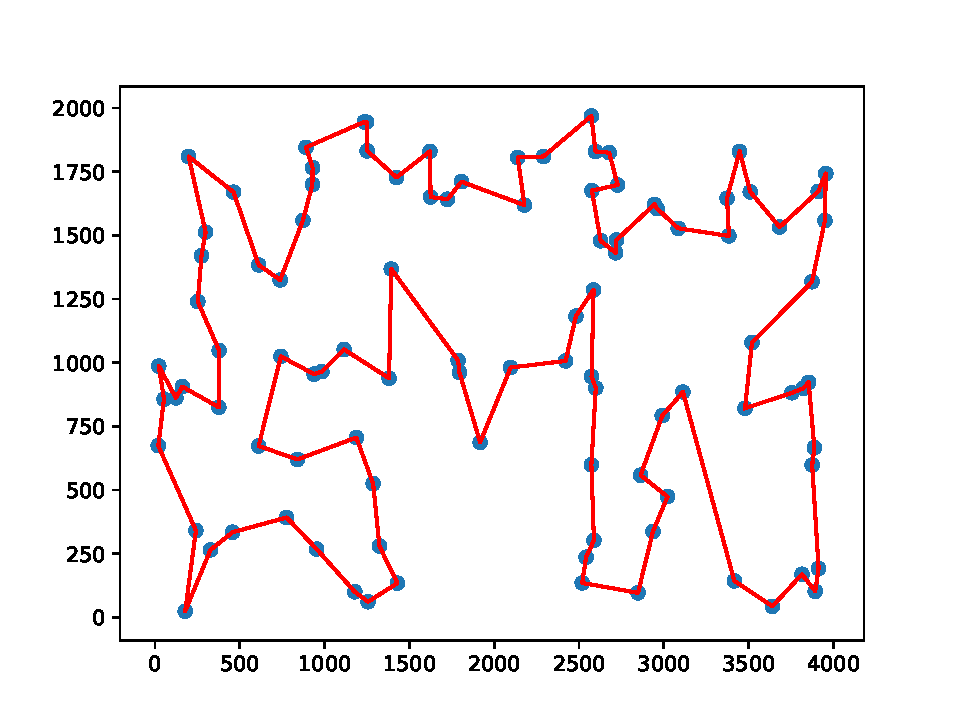
\includegraphics[scale = 0.44]{../../Implementation/gen/best_path_gtspams_kroA100}
		\label{fig:best_path_gtspams_kroA100}
		\caption{GTSPA-MS}
	\end{subfigure}
	\begin{subfigure}{.5\textwidth}
		\centering
		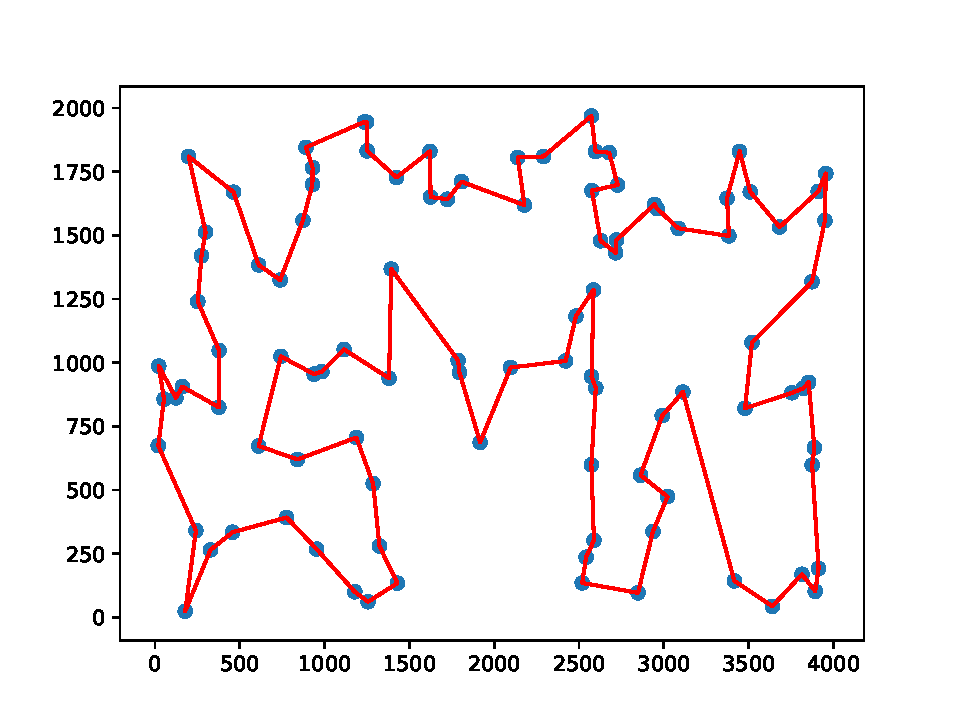
\includegraphics[scale = 0.44]{../../Implementation/gen/best_path_gtspasm_kroA100}
		\label{fig:best_path_gtspasm_kroA100}
		\caption{GTSPA-SM}
	\end{subfigure}%
	\begin{subfigure}{.5\textwidth}
		\centering
		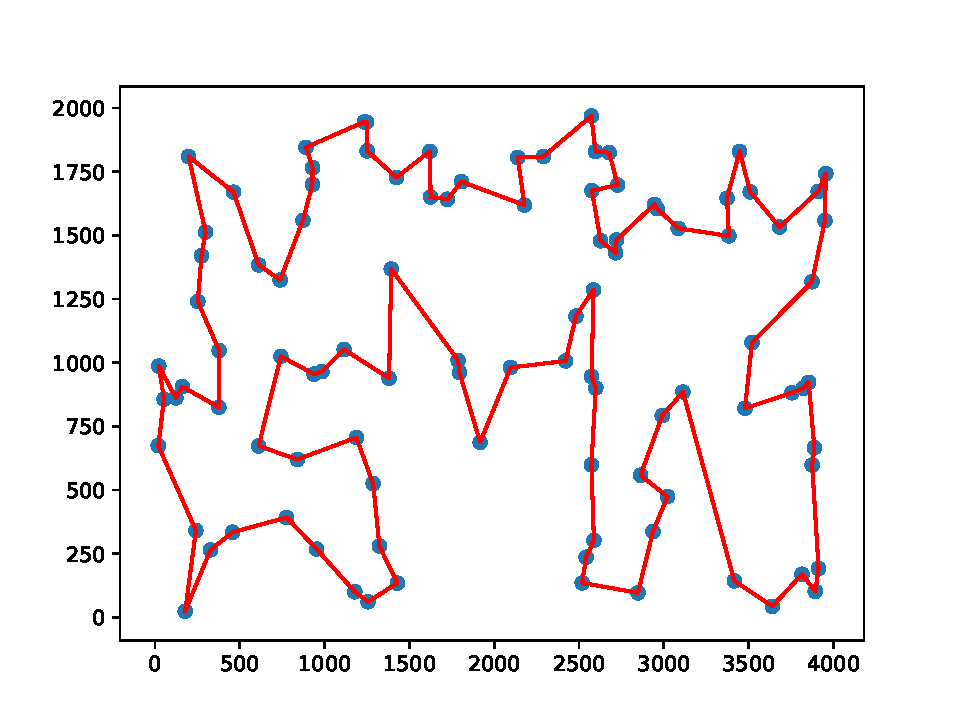
\includegraphics[scale = 0.44]{../../Implementation/gen/best_path_gtspasms_kroA100}
		\label{fig:best_path_gtspasms_kroA100}
		\caption{GTSPA-SMS}
	\end{subfigure}
	\begin{subfigure}{.5\textwidth}
		\centering
		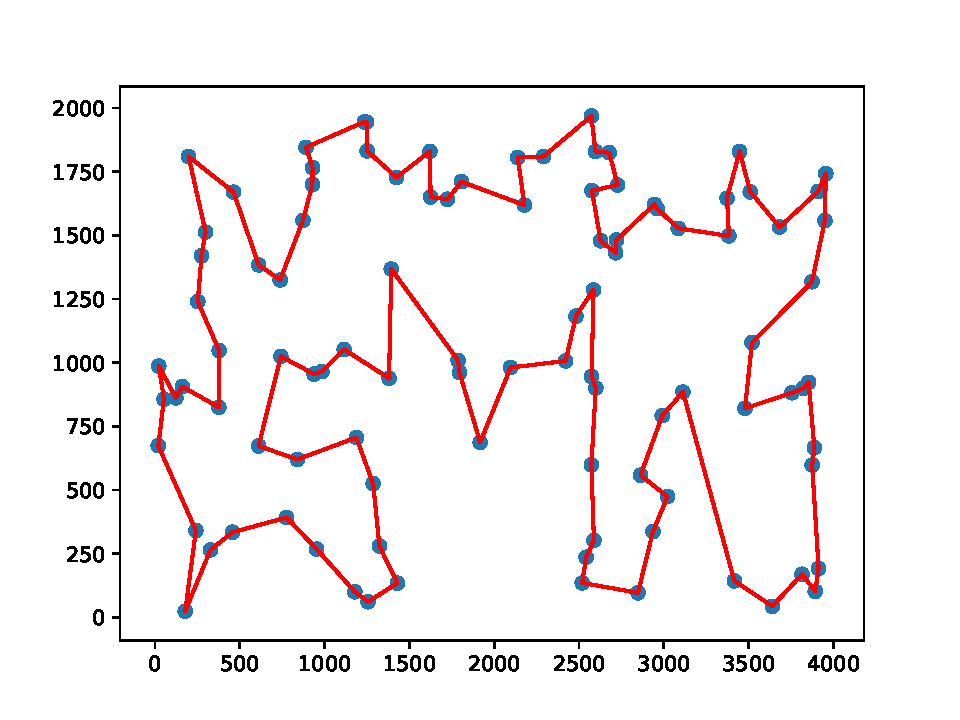
\includegraphics[scale = 0.44]{../../Implementation/gen/optimal_path_kroA100}
		\label{fig:optimal_path_kroA100}
		\caption{optimal path}
	\end{subfigure}
	\caption{Final best paths for the different algorithms and optimal path for 'kroA100' problem.}
	\label{fig:final_paths_kroA100}
\end{figure}
\newpage
\begin{figure}[ht]
	\centering
	\begin{subfigure}{.5\textwidth}
		\centering
		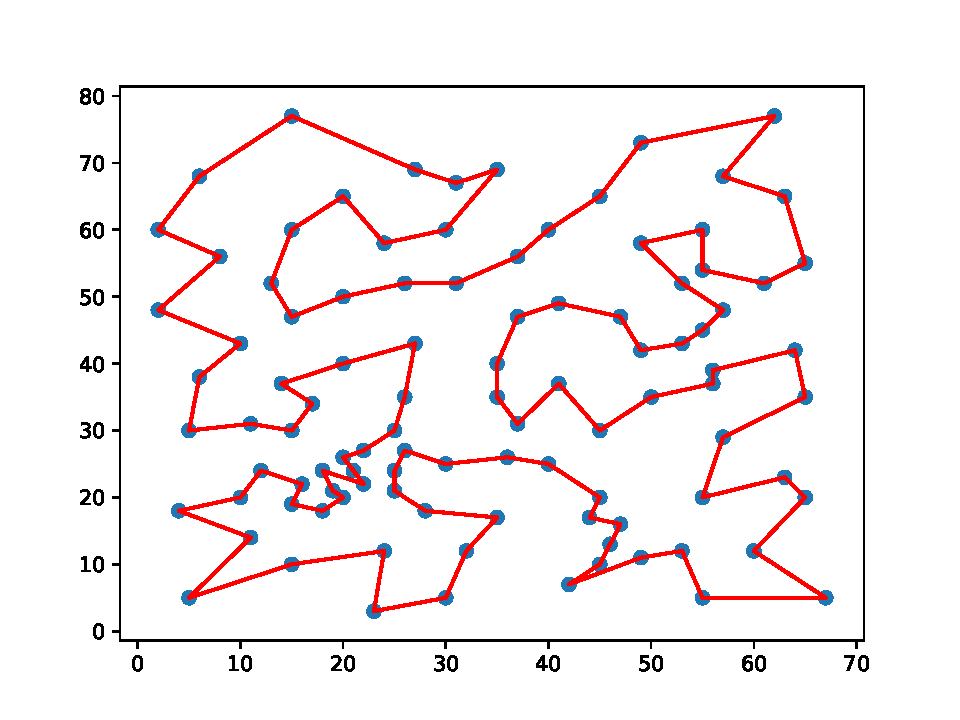
\includegraphics[scale = 0.44]{../../Implementation/gen/best_path_dtsa_eil101}
		\label{fig:best_path_dtsa_eil101}
		\caption{DTSA}
	\end{subfigure}%
	\begin{subfigure}{.5\textwidth}
		\centering
		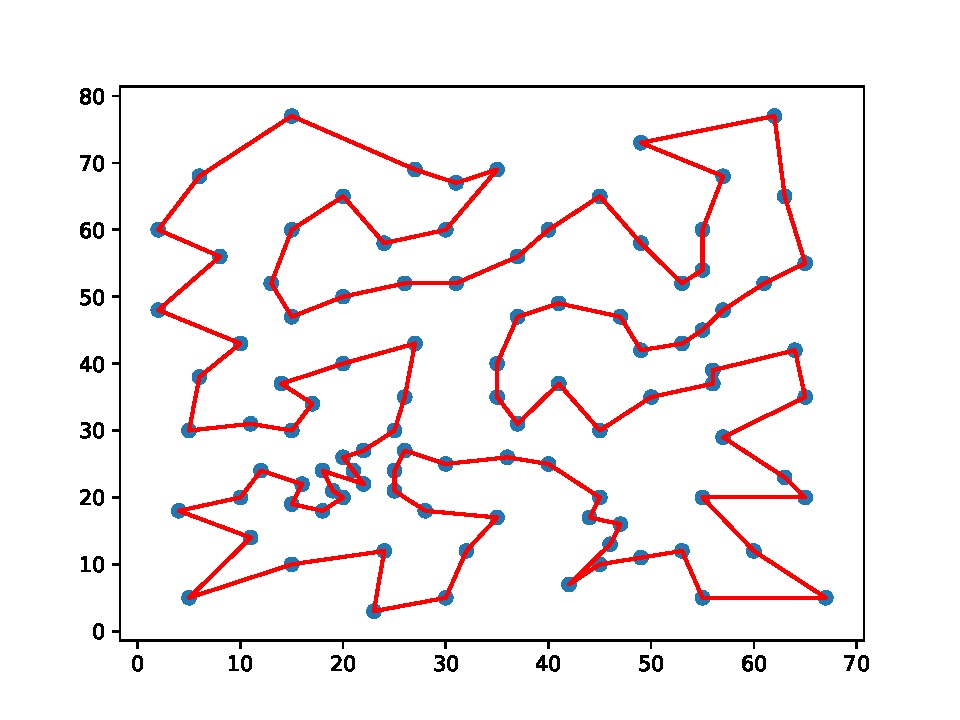
\includegraphics[scale = 0.44]{../../Implementation/gen/best_path_gtspams_eil101}
		\label{fig:best_path_gtspams_eil101}
		\caption{GTSPA-MS}
	\end{subfigure}
	\begin{subfigure}{.5\textwidth}
		\centering
		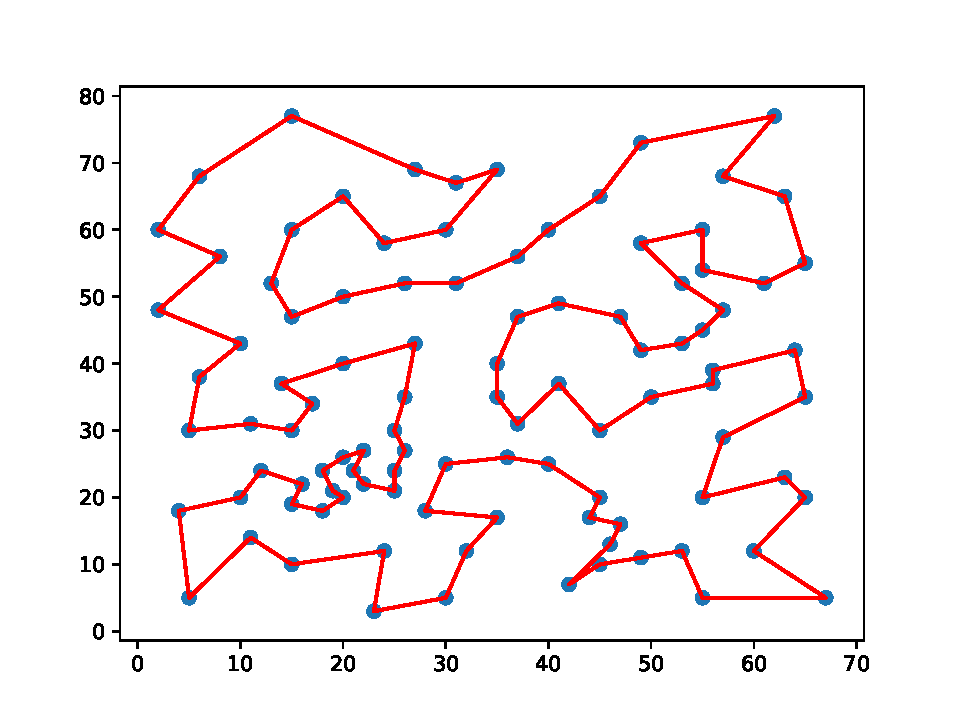
\includegraphics[scale = 0.44]{../../Implementation/gen/best_path_gtspasm_eil101}
		\label{fig:best_path_gtspasm_eil101}
		\caption{GTSPA-SM}
	\end{subfigure}%
	\begin{subfigure}{.5\textwidth}
		\centering
		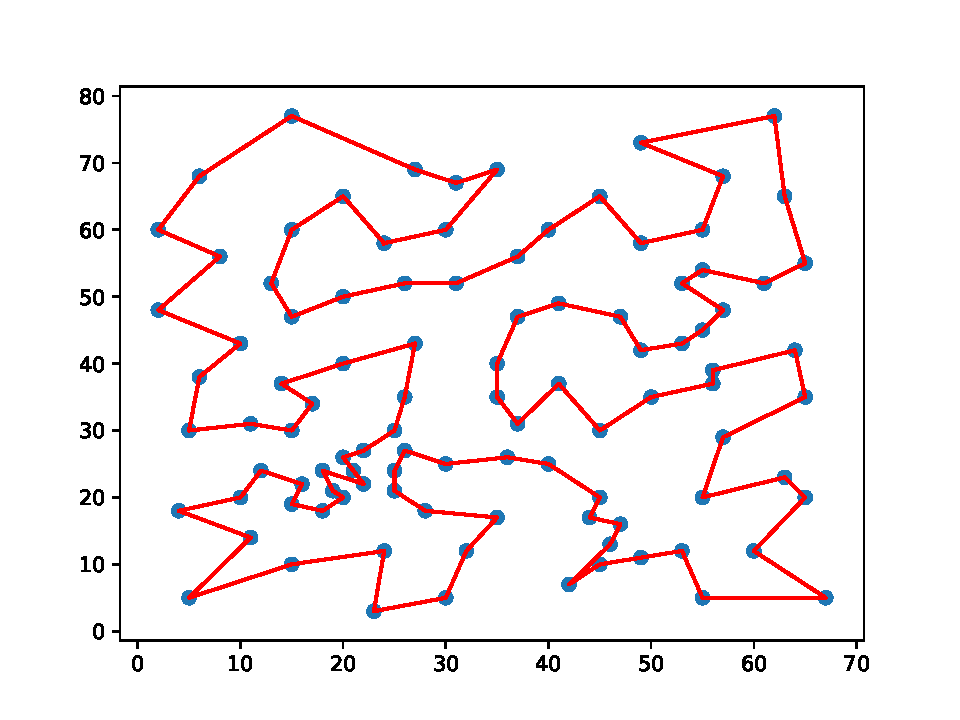
\includegraphics[scale = 0.44]{../../Implementation/gen/best_path_gtspasms_eil101}
		\label{fig:best_path_gtspasms_eil101}
		\caption{GTSPA-SMS}
	\end{subfigure}
	\begin{subfigure}{.5\textwidth}
		\centering
		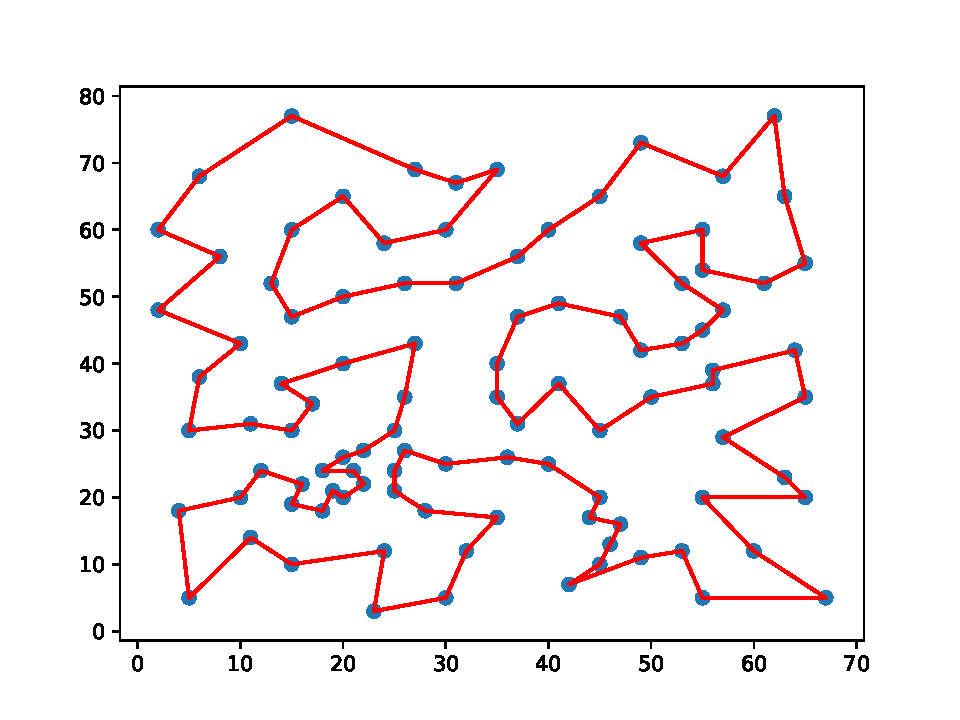
\includegraphics[scale = 0.44]{../../Implementation/gen/optimal_path_eil101}
		\label{fig:optimal_path_eil101}
		\caption{optimal path}
	\end{subfigure}
	\caption{Final best paths for the different algorithms and optimal path for 'eil101' problem.}
	\label{fig:final_paths_eil101}
\end{figure}
\newpage
\begin{figure}[ht]
	\centering
	\begin{subfigure}{.5\textwidth}
		\centering
		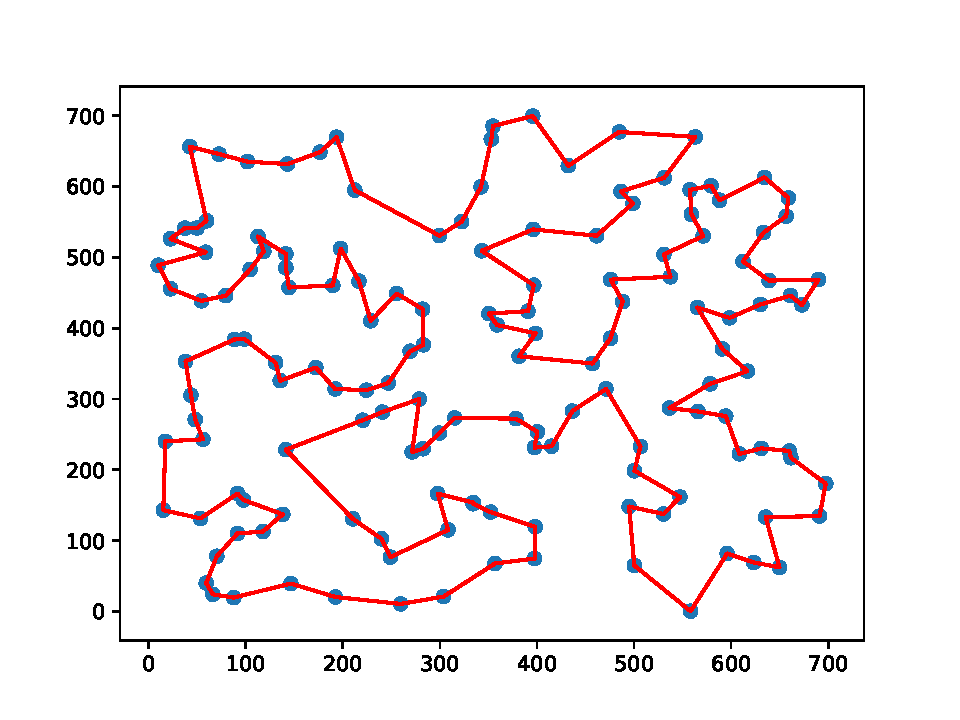
\includegraphics[scale = 0.44]{../../Implementation/gen/best_path_dtsa_ch150}
		\label{fig:best_path_dtsa_ch150}
		\caption{DTSA}
	\end{subfigure}%
	\begin{subfigure}{.5\textwidth}
		\centering
		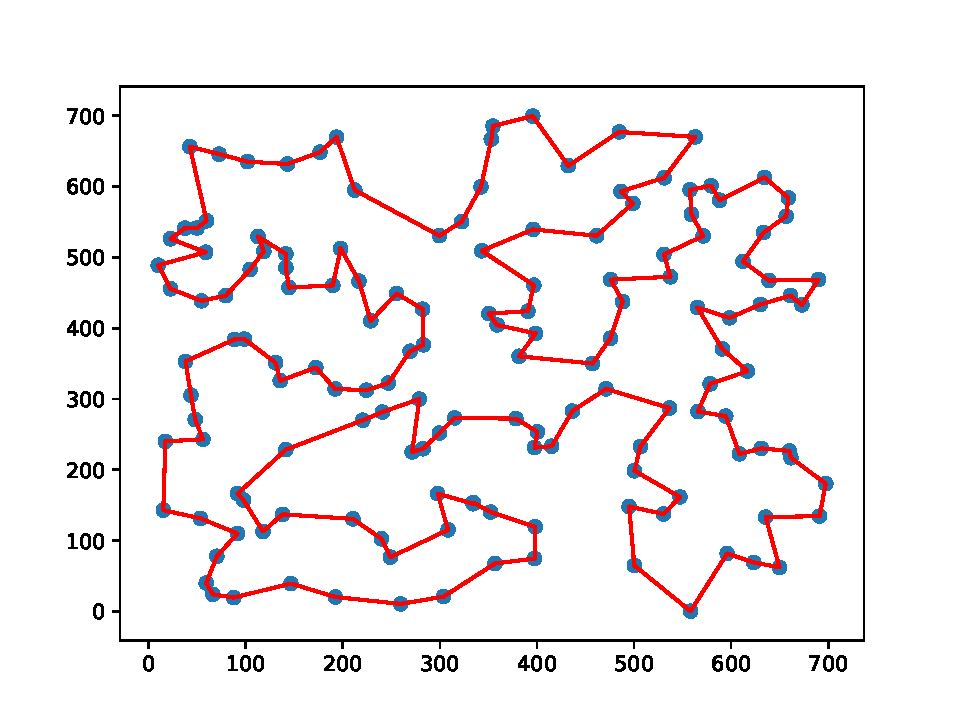
\includegraphics[scale = 0.44]{../../Implementation/gen/best_path_gtspams_ch150}
		\label{fig:best_path_gtspams_ch150}
		\caption{GTSPA-MS}
	\end{subfigure}
	\begin{subfigure}{.5\textwidth}
		\centering
		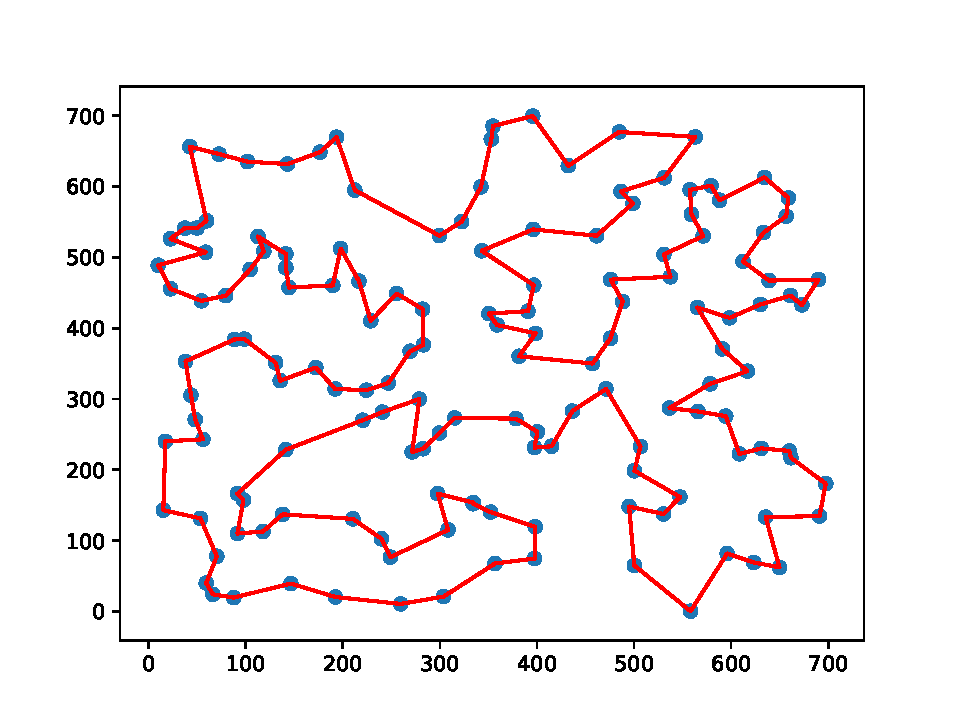
\includegraphics[scale = 0.44]{../../Implementation/gen/best_path_gtspasm_ch150}
		\label{fig:best_path_gtspasm_ch150}
		\caption{GTSPA-SM}
	\end{subfigure}%
	\begin{subfigure}{.5\textwidth}
		\centering
		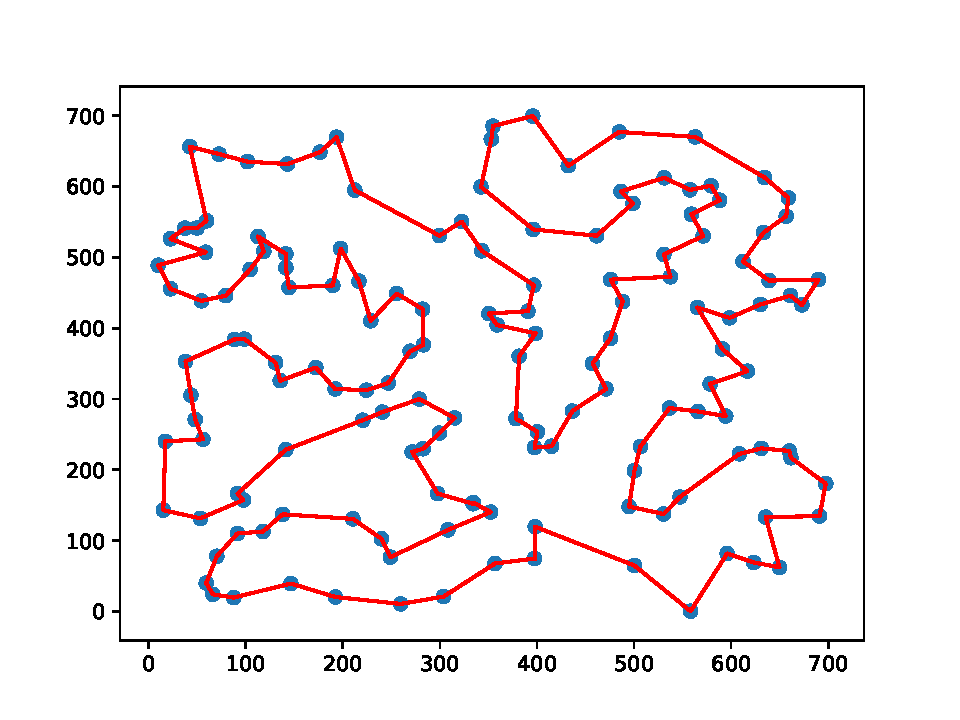
\includegraphics[scale = 0.44]{../../Implementation/gen/best_path_gtspasms_ch150}
		\label{fig:best_path_gtspasms_ch150}
		\caption{GTSPA-SMS}
	\end{subfigure}
	\begin{subfigure}{.5\textwidth}
		\centering
		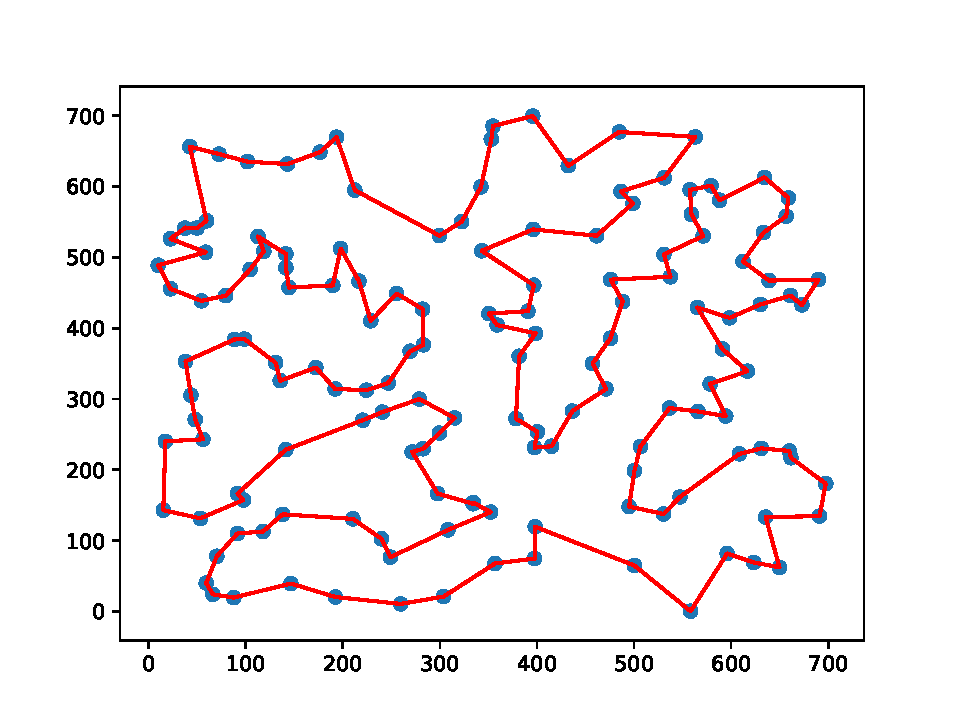
\includegraphics[scale = 0.44]{../../Implementation/gen/optimal_path_ch150}
		\label{fig:optimal_path_ch150}
		\caption{optimal path}
	\end{subfigure}
	\caption{Final best paths for the different algorithms and optimal path for 'ch150' problem.}
	\label{fig:final_paths_ch150}
\end{figure}
\newpage
\begin{figure}[ht]
	\centering
	\begin{subfigure}{.5\textwidth}
		\centering
		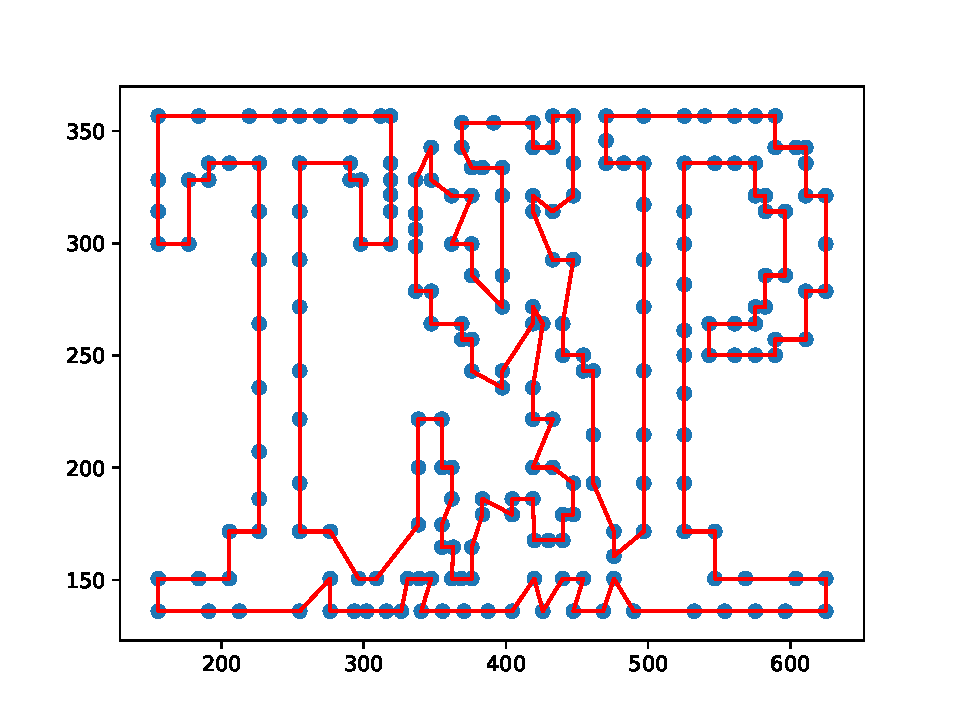
\includegraphics[scale = 0.44]{../../Implementation/gen/best_path_dtsa_tsp225}
		\label{fig:best_path_dtsa_tsp225}
		\caption{DTSA}
	\end{subfigure}%
	\begin{subfigure}{.5\textwidth}
		\centering
		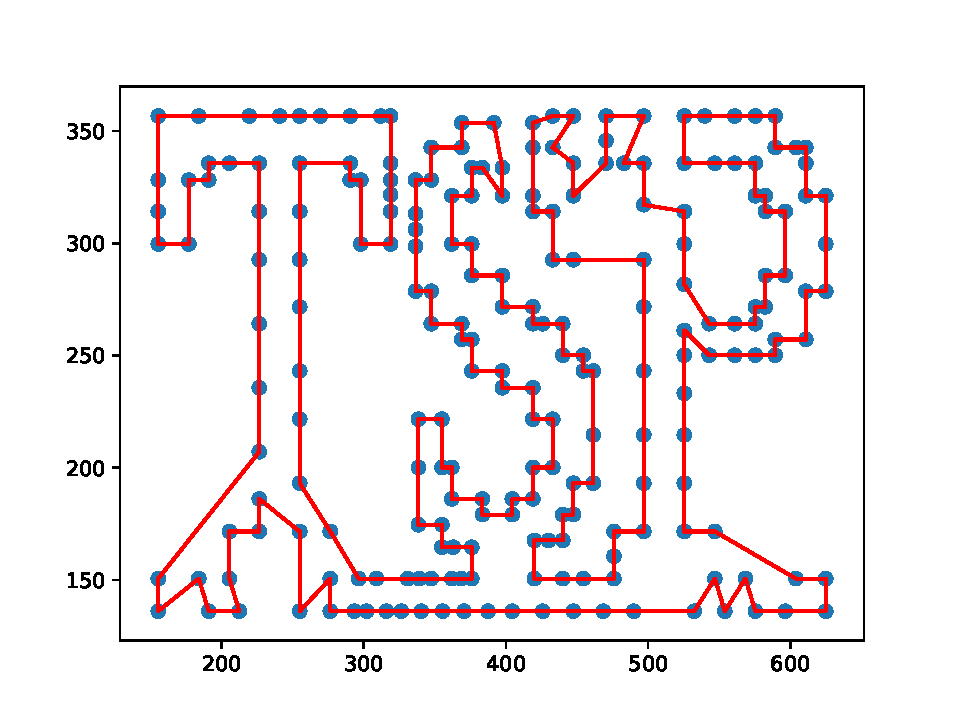
\includegraphics[scale = 0.44]{../../Implementation/gen/best_path_gtspams_tsp225}
		\label{fig:best_path_gtspams_tsp225}
		\caption{GTSPA-MS}
	\end{subfigure}
	\begin{subfigure}{.5\textwidth}
		\centering
		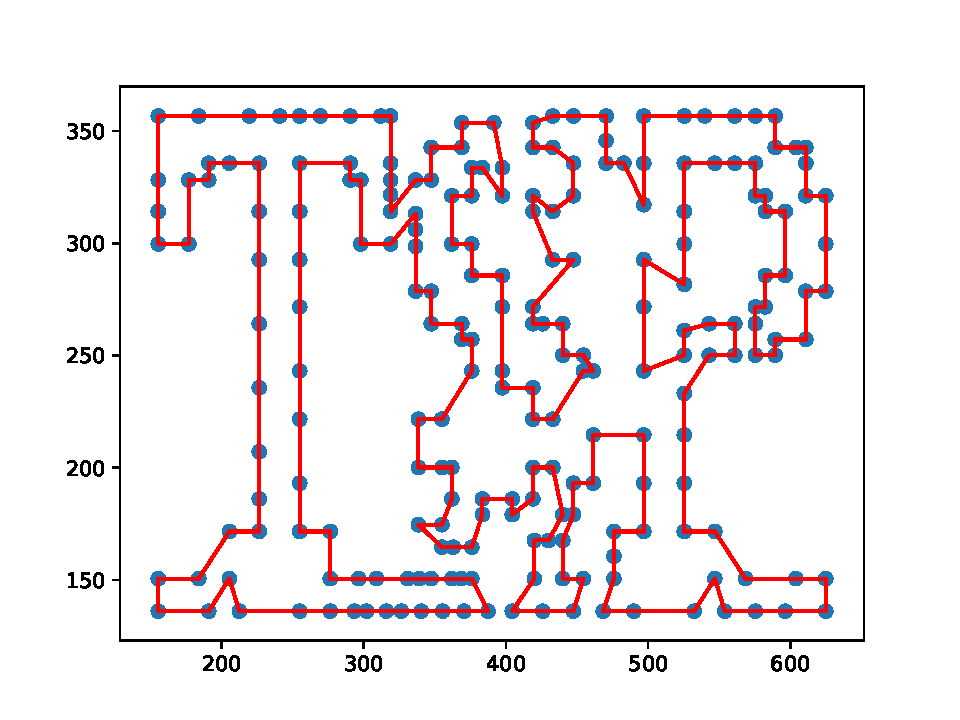
\includegraphics[scale = 0.44]{../../Implementation/gen/best_path_gtspasm_tsp225}
		\label{fig:best_path_gtspasm_tsp225}
		\caption{GTSPA-SM}
	\end{subfigure}%
	\begin{subfigure}{.5\textwidth}
		\centering
		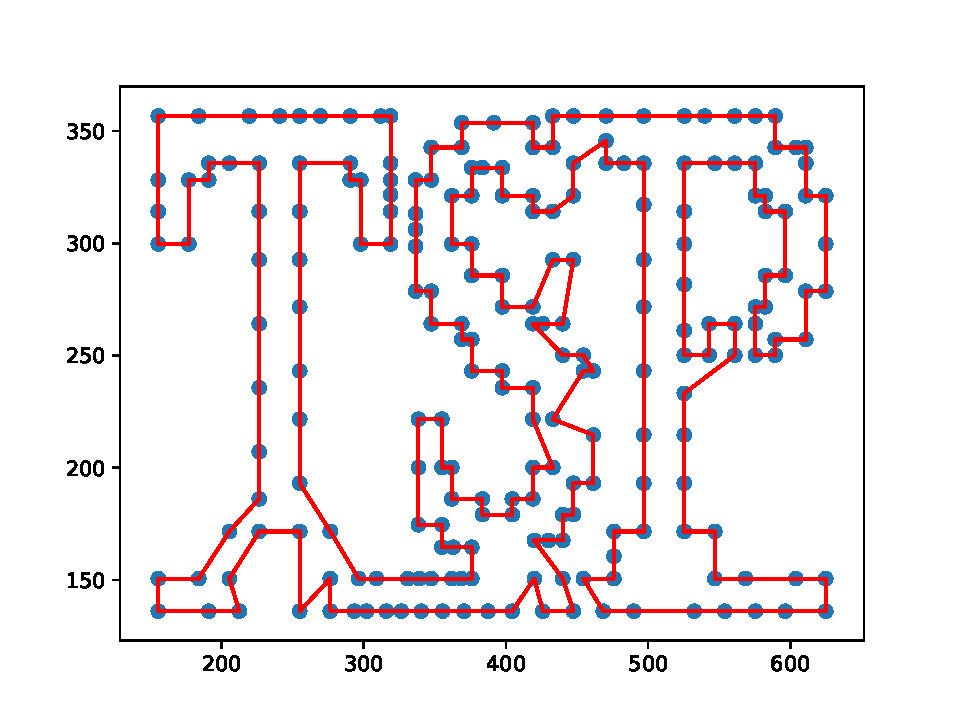
\includegraphics[scale = 0.44]{../../Implementation/gen/best_path_gtspasms_tsp225}
		\label{fig:best_path_gtspasms_tsp225}
		\caption{GTSPA-SMS}
	\end{subfigure}
	\begin{subfigure}{.5\textwidth}
		\centering
		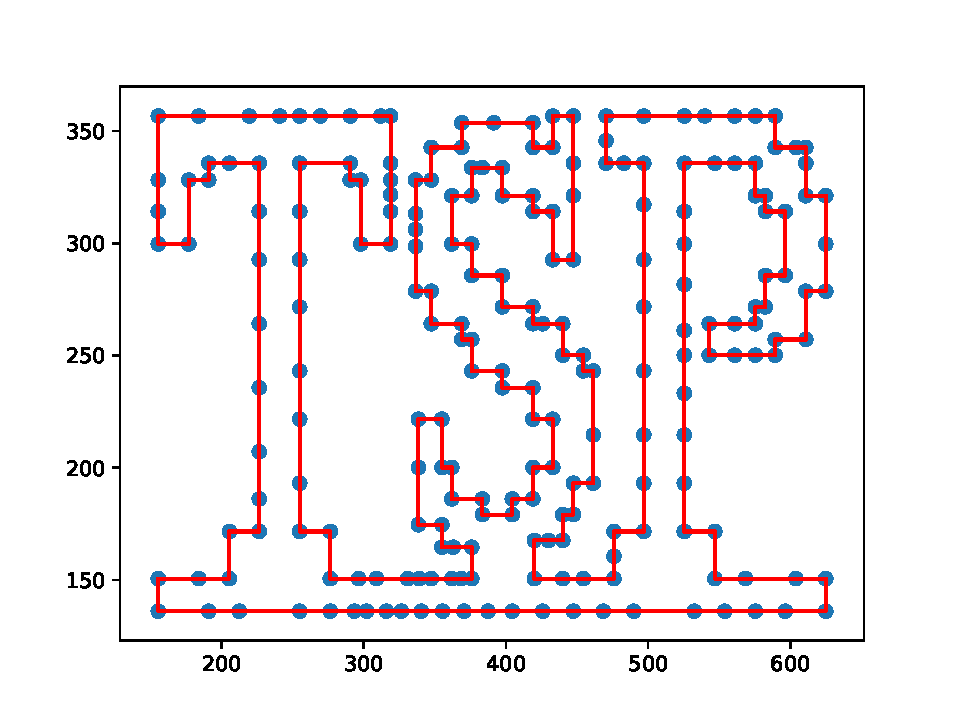
\includegraphics[scale = 0.44]{../../Implementation/gen/optimal_path_tsp225}
		\label{fig:optimal_path_tsp225}
		\caption{optimal path}
	\end{subfigure}
	\caption{Final best paths for the different algorithms and optimal path for 'tsp225' problem.}
	\label{fig:final_paths_tsp225}
\end{figure}

\newpage

\subsection{Source code}

Link to a git repository with full code:\\
\url{https://git.mafiasi.de/16beese/BAI-Seminar_Beese_Lohmann}

\end{document}